%Version 3.1 December 2024
%% CorePAM manuscript for Breast Cancer Research (BMC)
%% referee = double line spacing; lineno = continuous line numbering
%% sn-vancouver-num = Vancouver numbered references (BMC standard)
\documentclass[referee,lineno,pdflatex,sn-vancouver-num]{sn-jnl}

\usepackage{graphicx}
\usepackage{multirow}
\usepackage{amsmath,amssymb}
\usepackage{booktabs}
\usepackage{textcomp}
\usepackage{url}

\unnumbered% BCR: unnumbered section heads

\raggedbottom

\begin{document}

\title[CorePAM]{CorePAM: a 24-gene PAM50-derived expression score with cross-platform external validation for breast cancer prognosis}

\author*[1]{\fnm{Rafael} \spfx{de Negreiros} \sur{Botan}}\email{oncologista@gmail.com}

\author[2]{\fnm{Jo\~{a}o Batista} \spfx{de} \sur{Sousa}}

\affil*[1]{\orgdiv{Department of Oncology}, \orgname{Universidade de Bras\'{i}lia}, \orgaddress{\city{Bras\'{i}lia}, \country{Brazil}}}

\affil[2]{\orgdiv{Department of Proctology}, \orgname{Universidade de Bras\'{i}lia}, \orgaddress{\city{Bras\'{i}lia}, \country{Brazil}}}

\abstract{
\textbf{Background:} The PAM50 classifier predicts breast cancer prognosis but requires 50 genes and specialised platforms. We derived CorePAM, the smallest data-driven PAM50 subset maintaining non-inferior prognostic performance relative to a full 50-gene Cox elastic-net model, without pre-specifying gene count.

\textbf{Methods:} Cox elastic-net regression ($\alpha = 0.5$) with deterministic 10-fold cross-validation was applied in the SCAN-B cohort (N = 3,069; GSE96058). Gene selection followed a pre-specified non-inferiority margin ($\Delta$C-index = 0.010). External validation used four independent cohorts: TCGA-BRCA (N = 1,072; RNA-seq), METABRIC (N = 1,978; microarray; disease-specific survival), GSE20685 (N = 327; microarray), and GSE1456 (N = 159; microarray). Incremental value over a clinical model (CORE-A: age and ER status) was assessed by bootstrap $\Delta$C-index. Secondary analyses evaluated pathologic complete response (pCR) prediction in four neoadjuvant cohorts (N = 697) plus I-SPY2 (N = 986).

\textbf{Results:} CorePAM comprises 24 genes with an out-of-fold C-index of 0.670 (gap vs 50-gene maximum: 0.009). The score was independently associated with survival in all validation cohorts: TCGA-BRCA (HR = 1.20), METABRIC DSS (HR = 1.41), GSE20685 (HR = 1.40), GSE1456 (HR = 1.71); all $p < 0.02$. Random-effects meta-analysis (K = 4) yielded pooled HR = 1.37 (95\% CI 1.24--1.52; $I^2$ = 38.3\%; $p = 1.8 \times 10^{-9}$). CorePAM provided incremental value beyond CORE-A and remained significant after adjustment for T-stage and nodal status. For pCR, pooled OR = 1.69 (95\% CI 1.39--2.05; $I^2$ = 0\%; $p = 1.9 \times 10^{-7}$).

\textbf{Conclusions:} CorePAM---a 24-gene PAM50-derived score---achieves non-inferior discrimination relative to a 50-gene Cox elastic-net model across four validation cohorts spanning RNA-seq and microarray platforms, remains significant after anatomical staging adjustment, and predicts pCR. This reduction from 50 to 24 genes may facilitate implementation in resource-limited settings.
}

\keywords{Breast cancer \and Gene expression \and Prognostic signature \and PAM50 \and Elastic-net regression \and Survival analysis \and Pathologic complete response \and Cross-platform validation}

\maketitle

%% ============================================================
%%  BACKGROUND
%% ============================================================
\section{Background}\label{sec:background}

The PAM50 intrinsic subtype gene expression test classifies breast tumours into five molecular subtypes---Luminal~A, Luminal~B, HER2-enriched, Basal-like, and Normal-like~\cite{perou2000,sorlie2001}---and underpins the Prosigna prognostic assay~\cite{parker2009}. Its prognostic utility has been demonstrated across multiple independent cohorts and it is widely used for adjuvant chemotherapy decision-making in hormone receptor-positive, HER2-negative early breast cancer~\cite{cardoso2016,sparano2018}.

Despite its clinical validation, PAM50 requires simultaneous measurement of all 50 genes with calibrated reference samples. Its commercial implementation (Prosigna assay) is analytically validated exclusively on the NanoString nCounter platform~\cite{nielsen2014}, with substantial per-sample costs. These requirements create barriers in settings where RNA quality is limited (e.g., formalin-fixed paraffin-embedded tissue), platforms are unavailable, or per-sample costs are prohibitive. A reduced panel measurable by targeted RT-PCR or small targeted RNA-seq assays could extend the reach of molecular stratification to resource-limited settings. Existing reduced-gene assays such as the OncotypeDX Recurrence Score (21 genes)~\cite{paik2004} and the MammaPrint 70-gene signature~\cite{vantveer2002} were developed with different gene pools and endpoints; a PAM50-specific reduction has not been systematically attempted with modern penalised regression.

Previous attempts to reduce gene panels have typically pre-specified the target gene count before analysis, selected genes by threshold on univariate statistics, or used cohorts that mixed RNA-seq and microarray expression without platform-specific preprocessing. These approaches either introduce analytical circularity (optimising for the assumed answer) or ignore the multi-platform generalizability that clinical deployment demands.

We present CorePAM, a data-driven reduction of the PAM50 gene set derived from the complete SCAN-B RNA-seq cohort (N = 3,069) using elastic-net Cox regression with deterministic cross-validation and a pre-specified non-inferiority criterion relative to a full 50-gene Cox elastic-net model. Critically, the gene count was not pre-specified: it was derived entirely from the data and the pre-specified (a priori) and frozen $\Delta$C-index = 0.010 non-inferiority boundary. Validation was performed across four independent cohorts spanning one RNA-seq and three microarray platforms, including the largest publicly available microarray breast cancer cohort (METABRIC, N = 1,978). We further assessed whether CorePAM predicts pathologic complete response (pCR) to neoadjuvant chemotherapy---a clinical endpoint entirely distinct from the derivation analysis---in four independent neoadjuvant cohorts and the large I-SPY2 platform trial.

%% ============================================================
%%  METHODS
%% ============================================================
\section{Methods}\label{sec:methods}

\subsection{Study design}\label{subsec:study-design}

This is a retrospective multicohort study exclusively using publicly available de-identified data, reported following the TRIPOD guideline~\cite{moons2015}. No new data were collected. All analytical parameters were pre-specified and frozen before any analysis (see Analytical Freeze). External validation followed established principles for prognostic model assessment~\cite{royston2013}.

\subsection{Cohorts}\label{subsec:cohorts}

\textbf{Discovery cohort:} SCAN-B (GSE96058; N = 3,069 primary operable breast cancers)~\cite{brueffer2018,saal2015} provided RNA-seq data (Illumina paired-end sequencing) with matched clinical follow-up. All SCAN-B samples with eligible data were used for model development; no predefined training/validation split was provided in the public metadata.

\textbf{Validation cohorts (OS/DSS block):}

\begin{itemize}
\item \textit{TCGA-BRCA} (N = 1,072)~\cite{tcga2012}: RNA-seq (STAR aligner; GDC release); primary endpoint overall survival (OS).
\item \textit{METABRIC} (N = 1,978; cBioPortal)~\cite{curtis2012}: Illumina HT-12 microarray; primary endpoint disease-specific survival (DSS). Deaths from other causes were censored at time of death. OS was assessed as a sensitivity analysis.
\item \textit{GSE20685} (N = 327)~\cite{kao2011}: Affymetrix HGU133A microarray; primary endpoint OS.
\item \textit{GSE1456} (N = 159; Stockholm cohort)~\cite{pawitan2005}: Affymetrix HGU133A/B microarray; primary endpoint OS. Clinical covariates (age, ER status) were not available in the public annotation; CORE-A adjustment was not performed for this cohort.
\end{itemize}

\textbf{pCR block cohorts (secondary analysis, independent of OS block):}

\begin{itemize}
\item GSE25066 (N = 508)~\cite{hatzis2011}, GSE20194 (N = 278)~\cite{maqc2010}, GSE32646 (N = 154)~\cite{miyake2012}, I-SPY1/GSE22226 (N = 149)~\cite{esserman2012}: GEO microarray cohorts with pCR data from neoadjuvant chemotherapy trials. After applying eligibility criteria (available pCR outcome and expression data for CorePAM genes), 697 samples were included in the primary pCR analysis.
\item I-SPY2/GSE194040 (N = 986)~\cite{wolf2022}: exploratory external cohort; pre-treatment RNA-seq biopsies; multi-arm neoadjuvant trial; batch-corrected by the original consortium using ComBat.
\end{itemize}

All cohorts underwent independent harmonisation; no expression or clinical data were pooled across cohorts.

\subsection{Analytical freeze}\label{subsec:analytical-freeze}

The following parameters were pre-specified and frozen before any analysis was performed, archived in the study repository (Table~\ref{tab:freeze}).

\begin{table}[h]
\caption{CorePAM derivation parameters and frozen analytical settings.}\label{tab:freeze}
\begin{tabular}{@{}ll@{}}
\toprule
Parameter & Value \\
\midrule
Non-inferiority margin ($\Delta$C-index) & 0.010 \\
Elastic-net mixing parameter ($\alpha$) & 0.5 \\
Cross-validation folds (K) & 10 \\
Fold assignment & Deterministic (SHA-256 of patient ID) \\
Minimum gene coverage (validation) & 80\% \\
Time unit & months (days / 30.4375) \\
Gene count & Not pre-specified (derived from data) \\
\botrule
\end{tabular}
\end{table}

\subsection{Expression preprocessing}\label{subsec:expression-preprocessing}

All preprocessing was performed independently per cohort with no inter-cohort pooling or batch correction.

\textit{RNA-seq cohorts (SCAN-B, TCGA-BRCA):} Raw counts were filtered with edgeR::filterByExpr~\cite{robinson2010}, normalised by TMM, and transformed to log-CPM (prior.count = 1). Ensembl identifiers were mapped to official HGNC symbols via org.Hs.eg.db (offline annotation). In the case of multiple Ensembl IDs mapping to the same HGNC symbol, the identifier with the highest intra-cohort variance was retained.

\textit{Microarray cohorts (METABRIC, GSE20685, GSE1456):} Log2-scaled intensities from GEO Series Matrix files (pre-processed by the original data submitters) were used without additional normalisation. METABRIC identifiers were mapped via org.Hs.eg.db; GSE20685 and GSE1456 (Affymetrix HGU133A/B) via hgu133a.db. Six PAM50 genes lack probes on HGU133A (platform ceiling: 44/50 = 88\%, above the 80\% minimum); of these, two belong to the CorePAM panel in GSE20685 (GPR160, CXXC5; 22/24 = 91.7\%) and three in GSE1456 (GPR160, CXXC5, KRT17; 21/24 = 87.5\%), both above the 80\% minimum. METABRIC ER status was obtained from the cBioPortal clinical file (ER\_IHC column).

\textit{Score completeness:} When fewer than 24 CorePAM genes are available (e.g., GSE20685: 22/24 genes, 91.7\%), the score is computed over available genes only, with the denominator renormalised accordingly. Gene coverage is reported per cohort (Table~\ref{tab:coverage}); the pre-specified minimum of 80\% was met in all cases. Sensitivity to missing genes is further assessed in a leave-one-gene-out analysis (Additional file~9: Figure~S9).

\begin{table}[h]
\caption{CorePAM gene coverage by validation cohort.}\label{tab:coverage}
\begin{tabular}{@{}llccl@{}}
\toprule
Cohort & Platform & Genes present & Coverage (\%) & Missing genes \\
\midrule
SCAN-B & RNA-seq (Illumina) & 24/24 & 100 & --- \\
TCGA-BRCA & RNA-seq (STAR/GDC) & 23/24 & 95.8 & MIA \\
METABRIC & Illumina HT-12 microarray & 24/24 & 100 & --- \\
GSE20685 & Affymetrix HGU133A & 22/24 & 91.7 & GPR160, CXXC5 \\
GSE1456 & Affymetrix HGU133A/B & 21/24 & 87.5 & GPR160, CXXC5, KRT17 \\
\botrule
\end{tabular}
\end{table}

\subsection{CorePAM derivation}\label{subsec:corepam-derivation}

Cox elastic-net regression ($\alpha = 0.5$~\cite{zou2005,tibshirani1997}; glmnet package~\cite{friedman2010,simon2011}) was fitted in SCAN-B using a 10-fold cross-validation scheme. Fold assignment was \textit{deterministic}, based on the first eight hexadecimal digits of the SHA-256 hash of each patient identifier, with event-stratification. This deterministic fold assignment ensures exact reproducibility from first principles without dependence on a random seed as driver of gene selection.

Out-of-fold (OOF) C-index was computed for each degree-of-freedom level (df = number of non-zero genes) along the regularisation path. CorePAM was defined as the \textit{smallest df} satisfying: OOF C-index(df) $\geq$ OOF C-index(max) $-$ 0.010. The non-inferiority margin of 0.010 was chosen because it is less than half of one approximate standard error of the OOF C-index in the training cohort (SE $\approx$ 0.026 for N = 3,069 with 322 events), representing a clinically negligible loss in discrimination. Sensitivity analysis confirmed robustness: margins of 0.005, 0.015, and 0.020 would have selected 31, 18, and 16 genes respectively, demonstrating that the selected panel is not brittle to the choice of margin. Final model coefficients were extracted from the full-data path at the selected $\lambda$.

\subsection{Score calculation}\label{subsec:score-calculation}

For each cohort, the CorePAM score was computed as:
\begin{equation}
\text{score} = \frac{\sum_{i} w_i \cdot z_i}{\sum_{i} |w_i|}
\end{equation}
where the summation runs over the set of CorePAM genes present in the cohort ($G_{\text{present}}$), $z_i$ is the intra-cohort z-score of gene $i$, and $w_i$ is its elastic-net Cox regression weight from the frozen model. The score was subsequently standardised intra-cohort (score\_z = scale(score)) for proportional hazards regression, yielding hazard ratios per 1~SD. Score direction (positive = higher risk) was established in the SCAN-B training cohort (training HR = 1.92, confirming positive orientation); the same directional convention was confirmed to hold in all four external validation cohorts (all univariate HRs $> 1$) without requiring sign inversion in any cohort.

\subsection{Survival analysis}\label{subsec:survival-analysis}

\textbf{Univariate Cox:} score\_z as the sole predictor; HR per 1~SD with Wald confidence intervals.

\textbf{Multivariate Cox (CORE-A model):} score\_z adjusted for age (continuous) and ER status (binary), when ER was available in harmonised clinical data. CORE-A covariates by cohort: SCAN-B---age + ER status; METABRIC---age + ER status; TCGA-BRCA---age alone (ER status was not recoverable from the GDC-harmonised clinical file); GSE20685---age alone (ER status absent from the GSE Series Matrix clinical annotation). CORE-A denotes the clinical-only model (age $\pm$ ER).

\textbf{C-index:} Harrell's C-index~\cite{harrell1982} with 95\% bootstrap CI ($B = 1{,}000$). Uno's C-statistic (IPCW)~\cite{uno2011} was computed as a sensitivity analysis to address heterogeneous censoring; time-dependent AUC at fixed horizons (60 months; 24 months for TCGA-BRCA) was estimated via the timeROC package~\cite{blanche2013}.

\textbf{Kaplan--Meier:} dichotomised at the intra-cohort median. Cox HR for the dichotomised groups (High vs Low) with 95\% CI and Wald $p$-value are annotated on each figure. Quartile sensitivity analysis.

\textbf{Proportional hazards assumption:} The proportional hazards assumption was assessed graphically via scaled Schoenfeld residual plots and formally tested using the Grambsch--Therneau global test~\cite{grambsch1994} for each cohort. No significant departures were detected in SCAN-B, GSE20685, or GSE1456 (all global $p > 0.05$). METABRIC DSS showed marginal non-proportionality ($p = 0.04$), expected given its 159-month follow-up; the Fine--Gray competing-risks analysis and the concordance-based C-index (which does not assume proportional hazards) mitigate this concern.

\textbf{Fine--Gray competing risks~\cite{fine1999}:} applied to METABRIC DSS (deaths from other causes as competing event).

\textbf{Incremental value:} $\Delta$C-index = C(CORE-A + score\_z) $-$ C(CORE-A); bootstrap 95\% CI ($B = 1{,}000$).

\textbf{Meta-analysis:} Random-effects model using REML estimator for the OS/DSS block; DerSimonian--Laird~\cite{dersimonian1986} for the pCR block (metafor package~\cite{viechtbauer2010}). Heterogeneity was quantified using $I^2$~\cite{higgins2003}. Four independent validation cohorts were included (K = 4: TCGA-BRCA, METABRIC, GSE20685, GSE1456); SCAN-B excluded as training cohort. Hartung--Knapp adjustment~\cite{hartung2001} applied as sensitivity analysis.

\textbf{Calibration:} Formal calibration was assessed via logistic recalibration at the cohort-specific time horizon. Calibration intercept ($\alpha$; ideal = 0) and slope ($\beta$; ideal = 1) were obtained by regressing the binary outcome indicator $Y_H$ (event before horizon $H$) on the logit of the Cox-predicted risk at $H$. The expected-to-observed (E/O) ratio and Brier score were also computed.

\textbf{Frozen z-score sensitivity:} As a sensitivity analysis addressing single-sample scoring feasibility, the mean and standard deviation per gene were frozen from the SCAN-B training cohort and applied to all external validation cohorts instead of computing intra-cohort z-scores. No cohort-level re-standardisation (i.e.\ no \texttt{scale()}) was applied to the composite score, ensuring that each patient's score depends only on their own expression values and the frozen SCAN-B reference---as would occur in clinical deployment with a single specimen. Cox HR and C-index were compared between frozen and intra-cohort approaches on the same raw-score scale.

\textbf{Subgroup analysis:} ER-stratified Cox HR, C-index, and formal score$\times$ER interaction tests were performed in SCAN-B (OS; ER available in 94\%) and METABRIC (DSS; ER available in 98\%). These analyses were added post hoc in response to reviewer feedback; all other modelling choices remained frozen.

\textbf{Full clinical baseline:} As a secondary analysis, CorePAM was tested for incremental value beyond a comprehensive 6-variable clinical model (age + ER status + T-stage + N-status + grade + HER2 status) in SCAN-B and METABRIC---the two cohorts where all covariates were available. Complete-case analysis was used; reported sample sizes reflect patients with all six covariates available (SCAN-B: 2,649/3,069; METABRIC: 1,792/1,978). Incremental value was quantified by $\Delta$C-index (bootstrap $B = 1{,}000$) and a likelihood ratio test (LRT) comparing the clinical-only versus clinical + CorePAM models. This analysis was also performed restricted to ER-positive patients.

\textbf{Decision curve analysis (DCA)~\cite{vickers2006}:} Net benefit at clinically relevant probability thresholds using dcurves::dca (OS: 60-month horizon for SCAN-B, METABRIC, GSE20685; 24 months for TCGA-BRCA).

\textbf{Clinical baseline model scope:} CORE-A was pre-specified as the minimum clinical baseline (age and ER status) for consistency across cohorts, avoiding post-hoc covariate selection decisions. T-stage and nodal status were reserved for exploratory sensitivity analyses (Additional file~12: Table~S2), as their harmonisation quality varied across public data sources and their inclusion in the primary model would have introduced cohort-specific modelling decisions incompatible with a uniform validation framework.

\subsection{pCR analysis}\label{subsec:pcr-analysis}

Logistic regression: pCR $\sim$ score\_z (univariate); adjusted for age and ER/HER2 status where available. OR per 1~SD with Wald CI. AUC by DeLong method. Bootstrap CI ($B = 1{,}000$, seed = 42). I-SPY2 sensitivity analysis restricted to the paclitaxel control arm (N = 179).

\subsection{Quality control}\label{subsec:quality-control}

Comprehensive QC comprised: (i) off-diagonal score correlation between cohorts via percentile-based Pearson $r$; (ii) forensic PCA of METABRIC expression for batch effects and outliers; (iii) schema/range hard-checks on all analysis-ready files; (iv) automated anti-hardcoding assertions verifying all reported values against source CSV/JSON files.

\subsection{Data and code availability}\label{subsec:data-code}

All raw data are publicly available (GEO, GDC, cBioPortal). Analysis code is available at \url{https://github.com/RafaelBotan/CorePAM-Study}~\cite{botan2026}. All results are reproducible from the repository.

\subsection{Computational assistance}\label{subsec:computational-assistance}

A large language model (Claude, Anthropic) was used as a coding assistant for directory organisation, script development, and manuscript formatting. All code was reviewed and validated by the authors before use.

\subsection{Statistical software}\label{subsec:statistical-software}

R version 4.5.2. Key packages: glmnet~\cite{friedman2010} (elastic-net), survival~\cite{therneau2000}/survminer (Cox, KM), metafor~\cite{viechtbauer2010} (meta-analysis), dcurves (DCA), edgeR~\cite{robinson2010} (RNA-seq normalisation), genefu~\cite{gendoo2016} (signature comparison), survC1 (Uno's C-statistic), timeROC~\cite{blanche2013} (time-dependent AUC).

%% ============================================================
%%  RESULTS
%% ============================================================
\section{Results}\label{sec:results}

\subsection{CorePAM derivation}\label{subsec:results-derivation}

Out-of-fold Cox elastic-net regression in SCAN-B identified 24 genes as the minimum set satisfying the pre-specified non-inferiority criterion ($\Delta$C = 0.010). The selected model achieved an OOF C-index of 0.670, compared to the maximum OOF C-index achievable with all 50 PAM50 candidates (0.679), with a gap of 0.009---within the 0.010 boundary. The selected 24 genes and their elastic-net Cox weights are illustrated in Additional file~2: Figure~S2 and listed in Additional file~11: Table~S1.

\begin{figure}[p]
\centering

\includegraphics[width=\textwidth,height=0.85\textheight,keepaspectratio]{figures/Fig1_StudyDesign_EN.png}
\caption{Study design overview. CorePAM: a 24-gene prognostic signature derived from the PAM50 gene set via elastic-net Cox regression in SCAN-B (N = 3,069; RNA-seq) and validated in four independent cohorts (TCGA-BRCA, METABRIC, GSE20685, GSE1456; total N = 3,536) spanning RNA-seq and microarray platforms, plus five neoadjuvant chemotherapy cohorts for pCR prediction. All analytical parameters were pre-specified and frozen before analysis.}\label{fig:study-design}
\end{figure}

The 24 genes span luminal differentiation (ESR1, PGR, NAT1), proliferation (MYBL2, PTTG1, EXO1, MYC), basal phenotype (KRT5, KRT17, FOXC1), and HER2-enriched markers (ERBB2, GRB7, MIA), with full gene list in Additional file~11: Table~S1. The Pareto frontier (Additional file~1: Figure~S1) shows diminishing returns beyond approximately 15 genes, with the non-inferiority boundary crossed at df = 24. Bootstrap resampling ($B = 200$) confirmed that 15 of 24 CorePAM genes were selected in at least 70\% of resamples, with a minimum selection frequency of 35.5\% (Additional file~8: Figure~S8).

\subsection{Prognostic validation}\label{subsec:results-validation}

The CorePAM score was independently associated with survival in all four external validation cohorts (Table~\ref{tab:survival}). In TCGA-BRCA (RNA-seq), HR per 1~SD = 1.20 (95\% CI 1.04--1.40; $p = 0.016$). In METABRIC (DSS endpoint; Illumina microarray), HR = 1.41 (95\% CI 1.31--1.52; $p < 0.001$). In GSE20685 (Affymetrix microarray), HR = 1.40 (95\% CI 1.12--1.76; $p = 0.003$). In GSE1456 (Stockholm; Affymetrix microarray), HR = 1.71 (95\% CI 1.23--2.38; $p = 0.001$). Kaplan--Meier curves stratified at the intra-cohort median score are shown in Figures~\ref{fig:km-tcga}--\ref{fig:km-gse1456}.

\begin{table}[h]
\caption{CorePAM prognostic performance across cohorts.}\label{tab:survival}
\small
\begin{tabular*}{\textwidth}{@{\extracolsep\fill}lcrrllll}
\toprule
Cohort & Endpoint & N & Events & Univariate HR & Adjusted HR\footnotemark[1] & C-index \\
\midrule
SCAN-B\footnotemark[2] & OS & 3,069 & 322 & 1.92 (1.74--2.13) & 1.86 (1.64--2.12) & 0.698 (0.668--0.729) \\
TCGA-BRCA & OS & 1,072 & 150 & 1.20 (1.04--1.40) & 1.27 (1.09--1.48) & 0.624 (0.572--0.678) \\
METABRIC & DSS & 1,978 & 646 & 1.41 (1.31--1.52) & 1.36 (1.24--1.48) & 0.638 (0.615--0.659) \\
GSE20685 & OS & 327 & 83 & 1.40 (1.12--1.76) & 1.40 (1.12--1.76) & 0.623 (0.562--0.683) \\
GSE1456\footnotemark[3] & OS & 159 & 40 & 1.71 (1.23--2.38) & --- & 0.661 (0.582--0.741) \\
\botrule
\end{tabular*}
\footnotetext{HR: hazard ratio per 1~SD (95\% CI); all $p < 0.02$.}
\footnotetext[1]{CORE-A: age + ER (SCAN-B, METABRIC); age only (TCGA-BRCA, GSE20685).}
\footnotetext[2]{Training cohort. C-index is in-sample (0.698); OOF C-index = 0.670.}
\footnotetext[3]{Clinical covariates unavailable; CORE-A adjustment not performed.}
\end{table}

\begin{figure}[h]
\centering
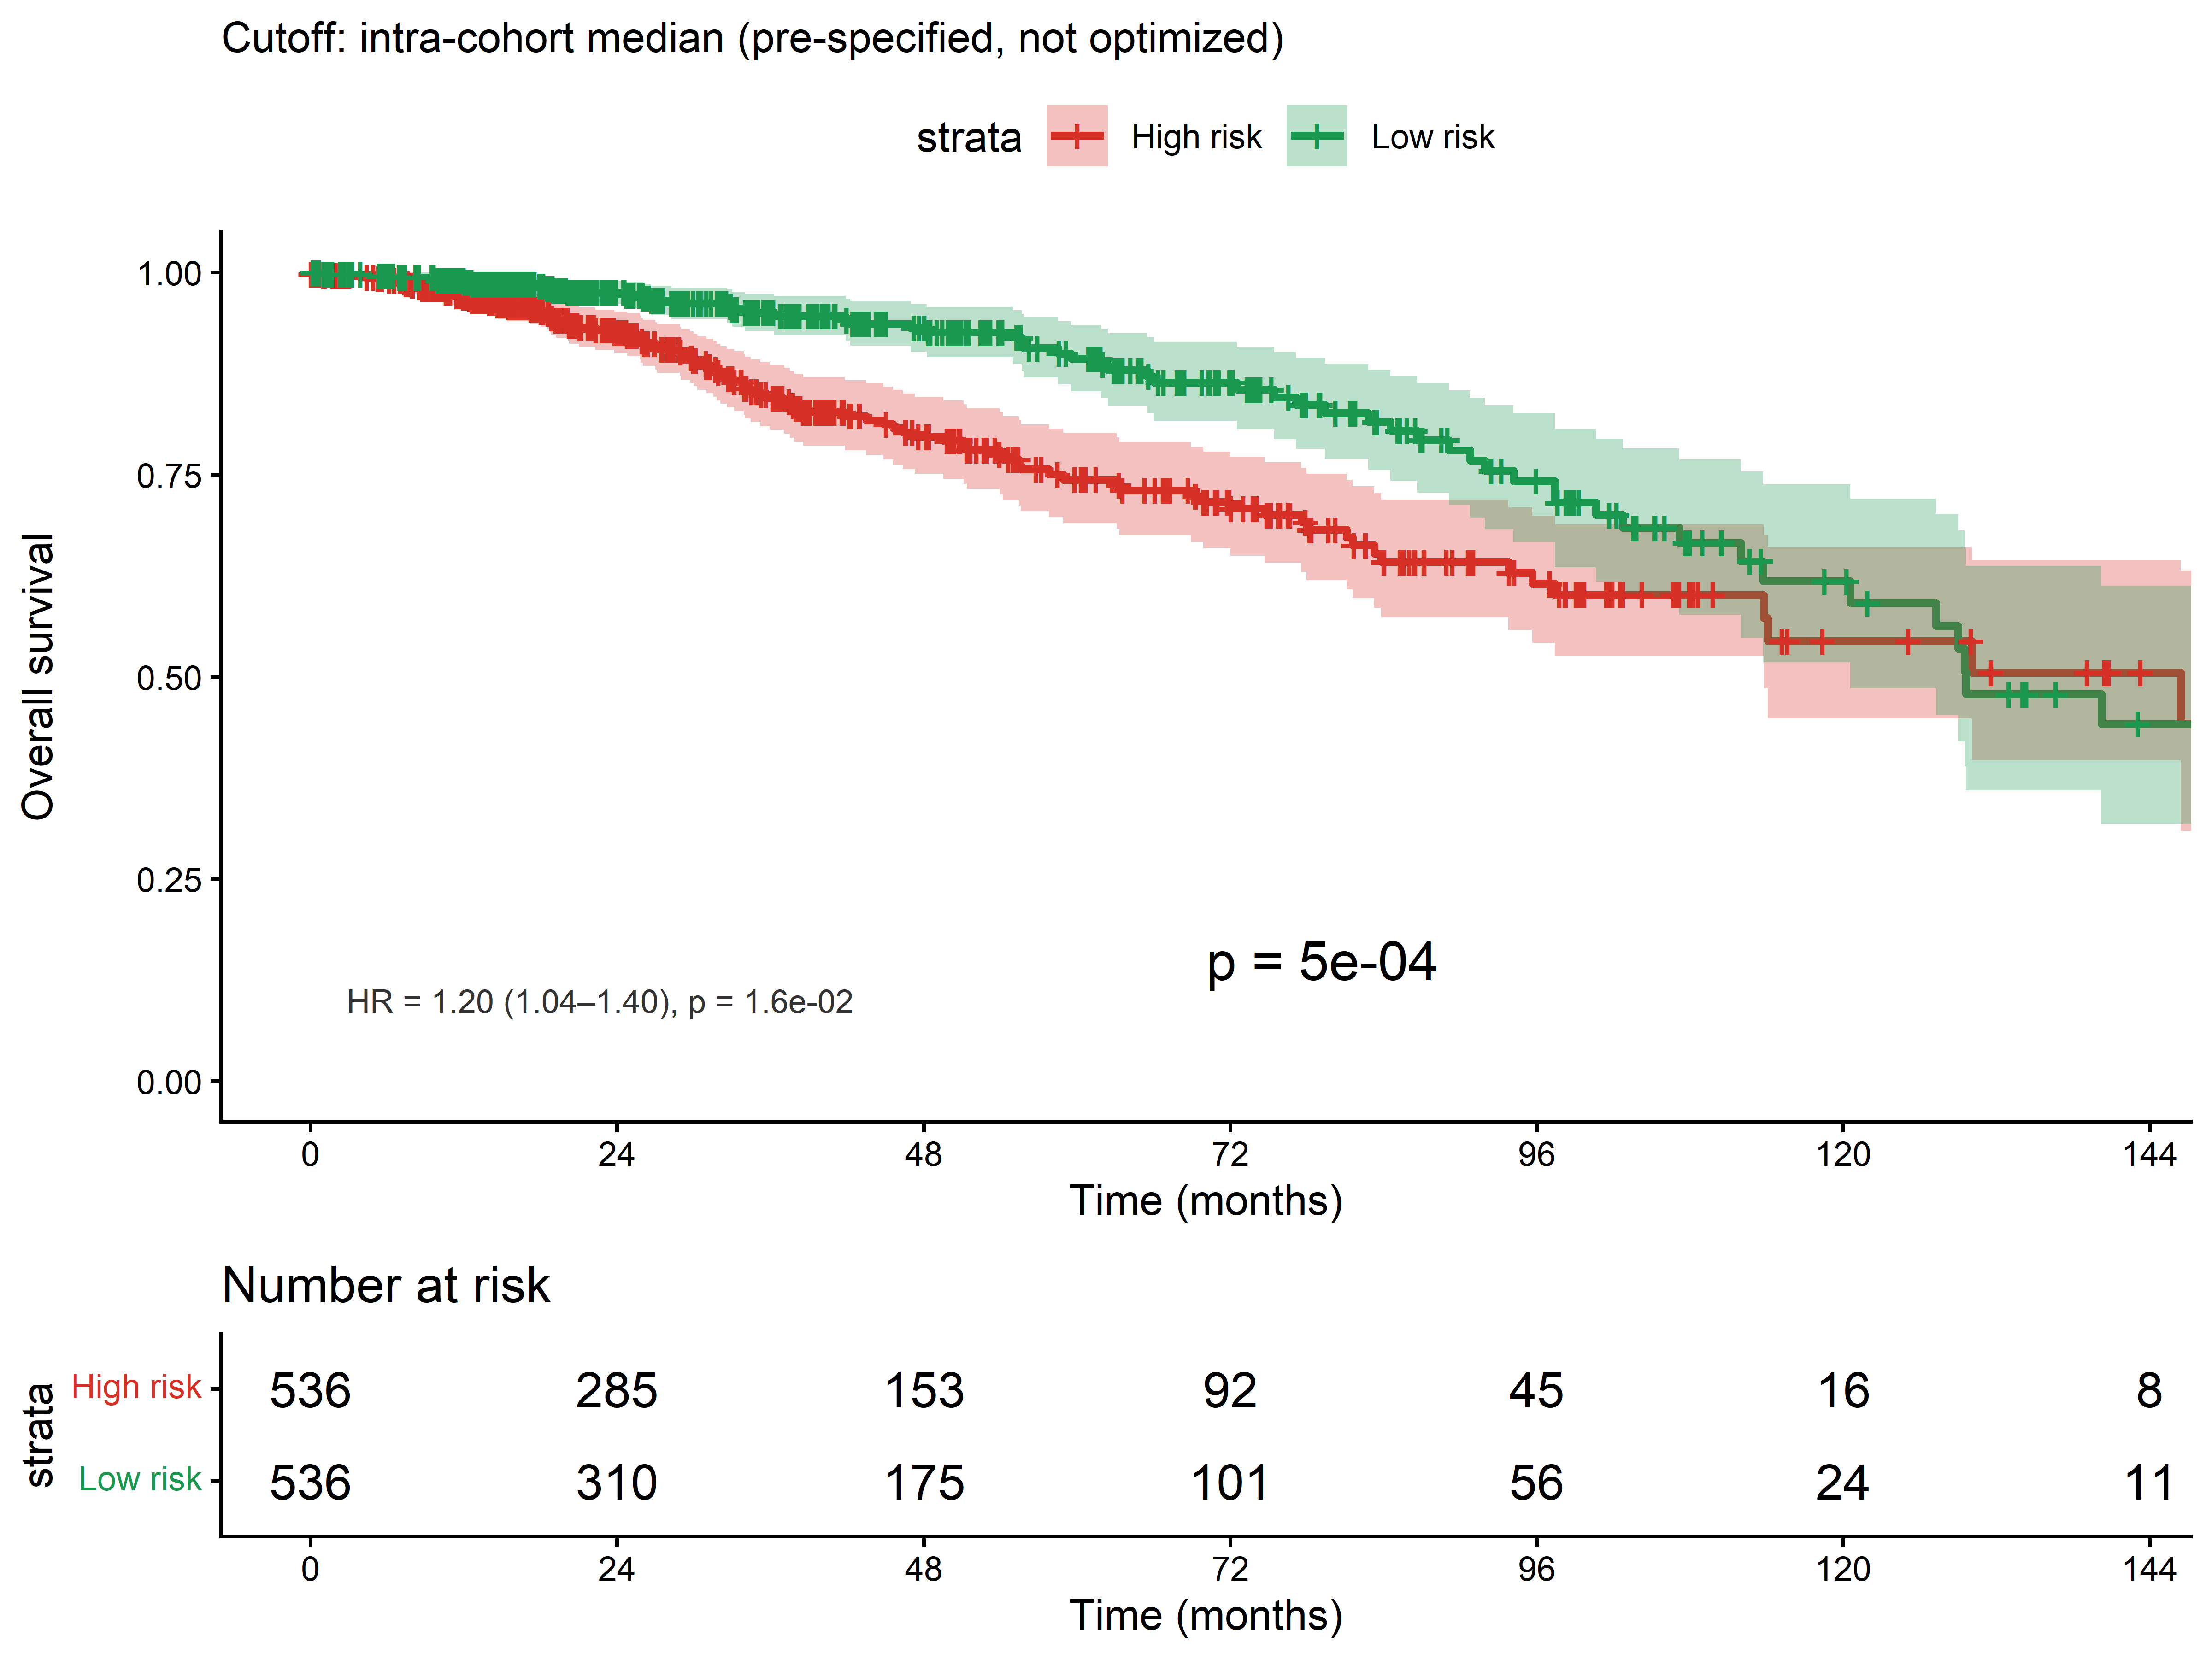
\includegraphics[width=\textwidth]{figures/Fig2_KM_TCGA_BRCA_OS_EN.png}
\caption{Kaplan--Meier overall survival curve in TCGA-BRCA (N = 1,072; 150 events; RNA-seq). Patients dichotomised at the intra-cohort median CorePAM score (High vs Low). Cox HR for the dichotomised groups with 95\% CI and Wald $p$-value annotated. Shading: 95\% CI.}\label{fig:km-tcga}
\end{figure}

\begin{figure}[h]
\centering

\includegraphics[width=\textwidth]{figures/Fig2_KM_METABRIC_DSS_EN.png}
\caption{Kaplan--Meier disease-specific survival curve in METABRIC (N = 1,978; 646 events; Illumina microarray). Patients dichotomised at the intra-cohort median CorePAM score (High vs Low). Cox HR for the dichotomised groups with 95\% CI and Wald $p$-value annotated. Shading: 95\% CI.}\label{fig:km-metabric}
\end{figure}

\begin{figure}[h]
\centering
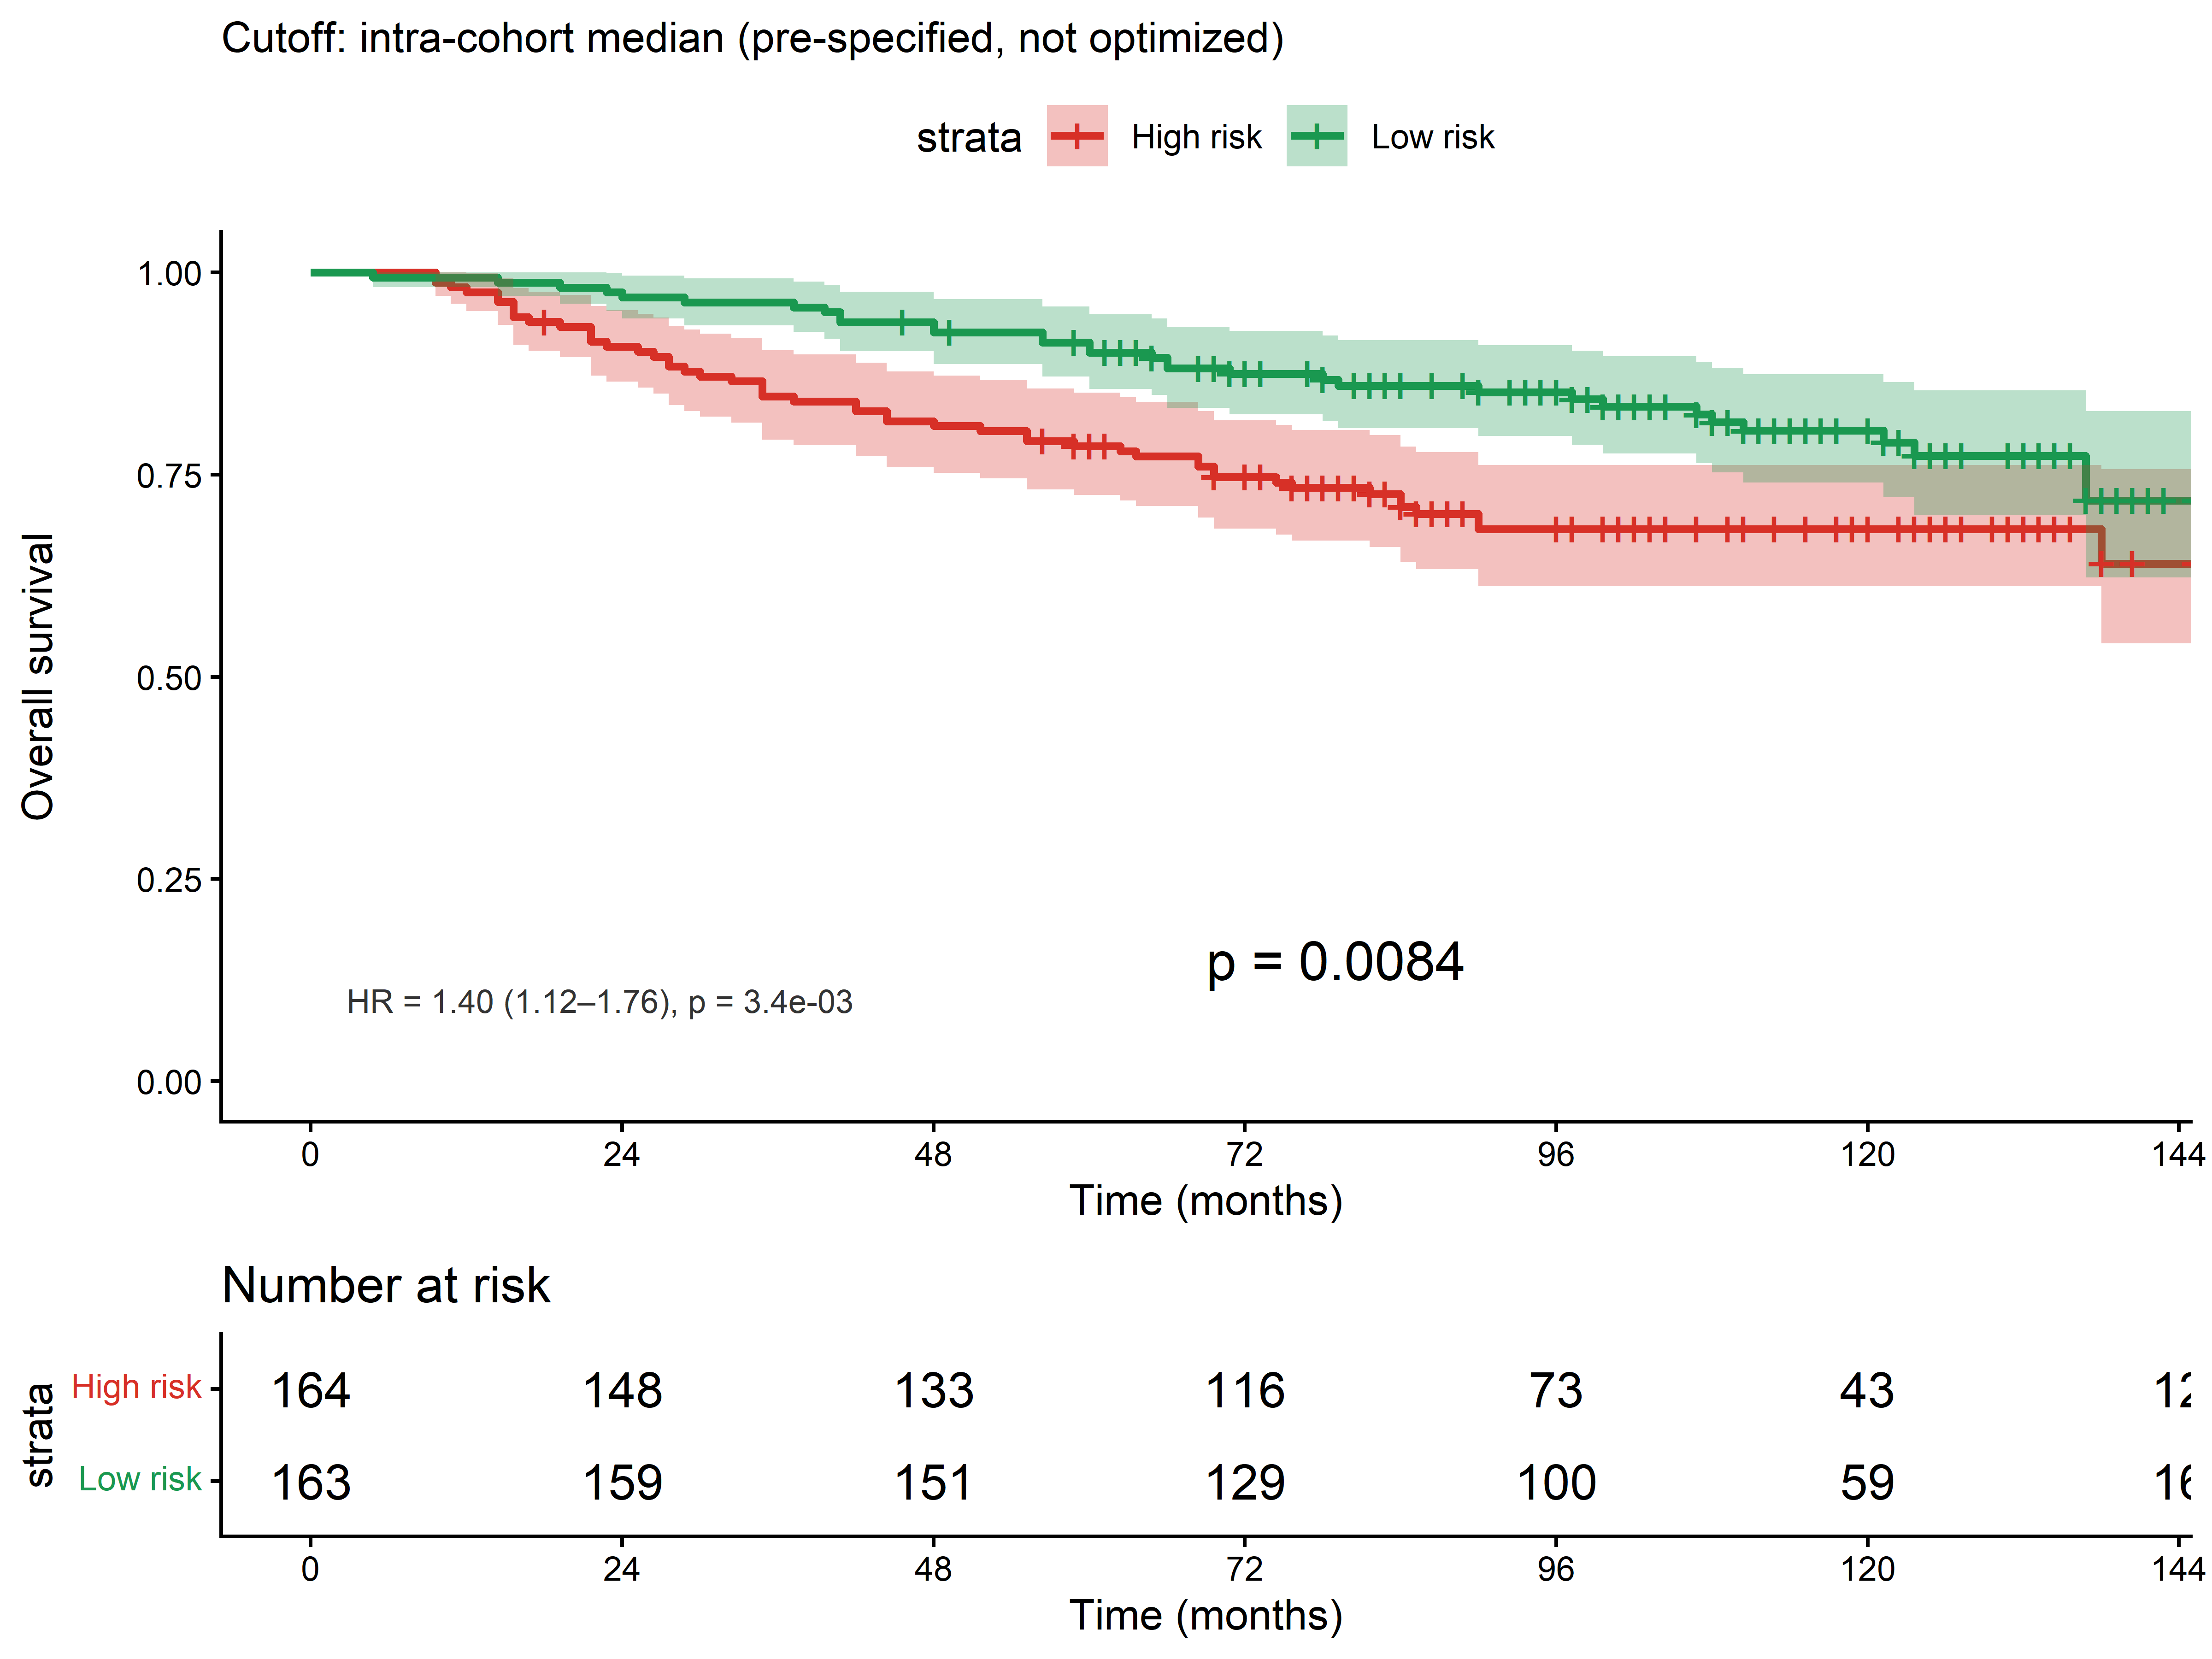
\includegraphics[width=\textwidth]{figures/Fig2_KM_GSE20685_OS_EN.png}
\caption{Kaplan--Meier overall survival curve in GSE20685 (N = 327; 83 events; Affymetrix microarray). Patients dichotomised at the intra-cohort median CorePAM score (High vs Low). Cox HR for the dichotomised groups with 95\% CI and Wald $p$-value annotated. Shading: 95\% CI.}\label{fig:km-gse20685}
\end{figure}

\begin{figure}[h]
\centering
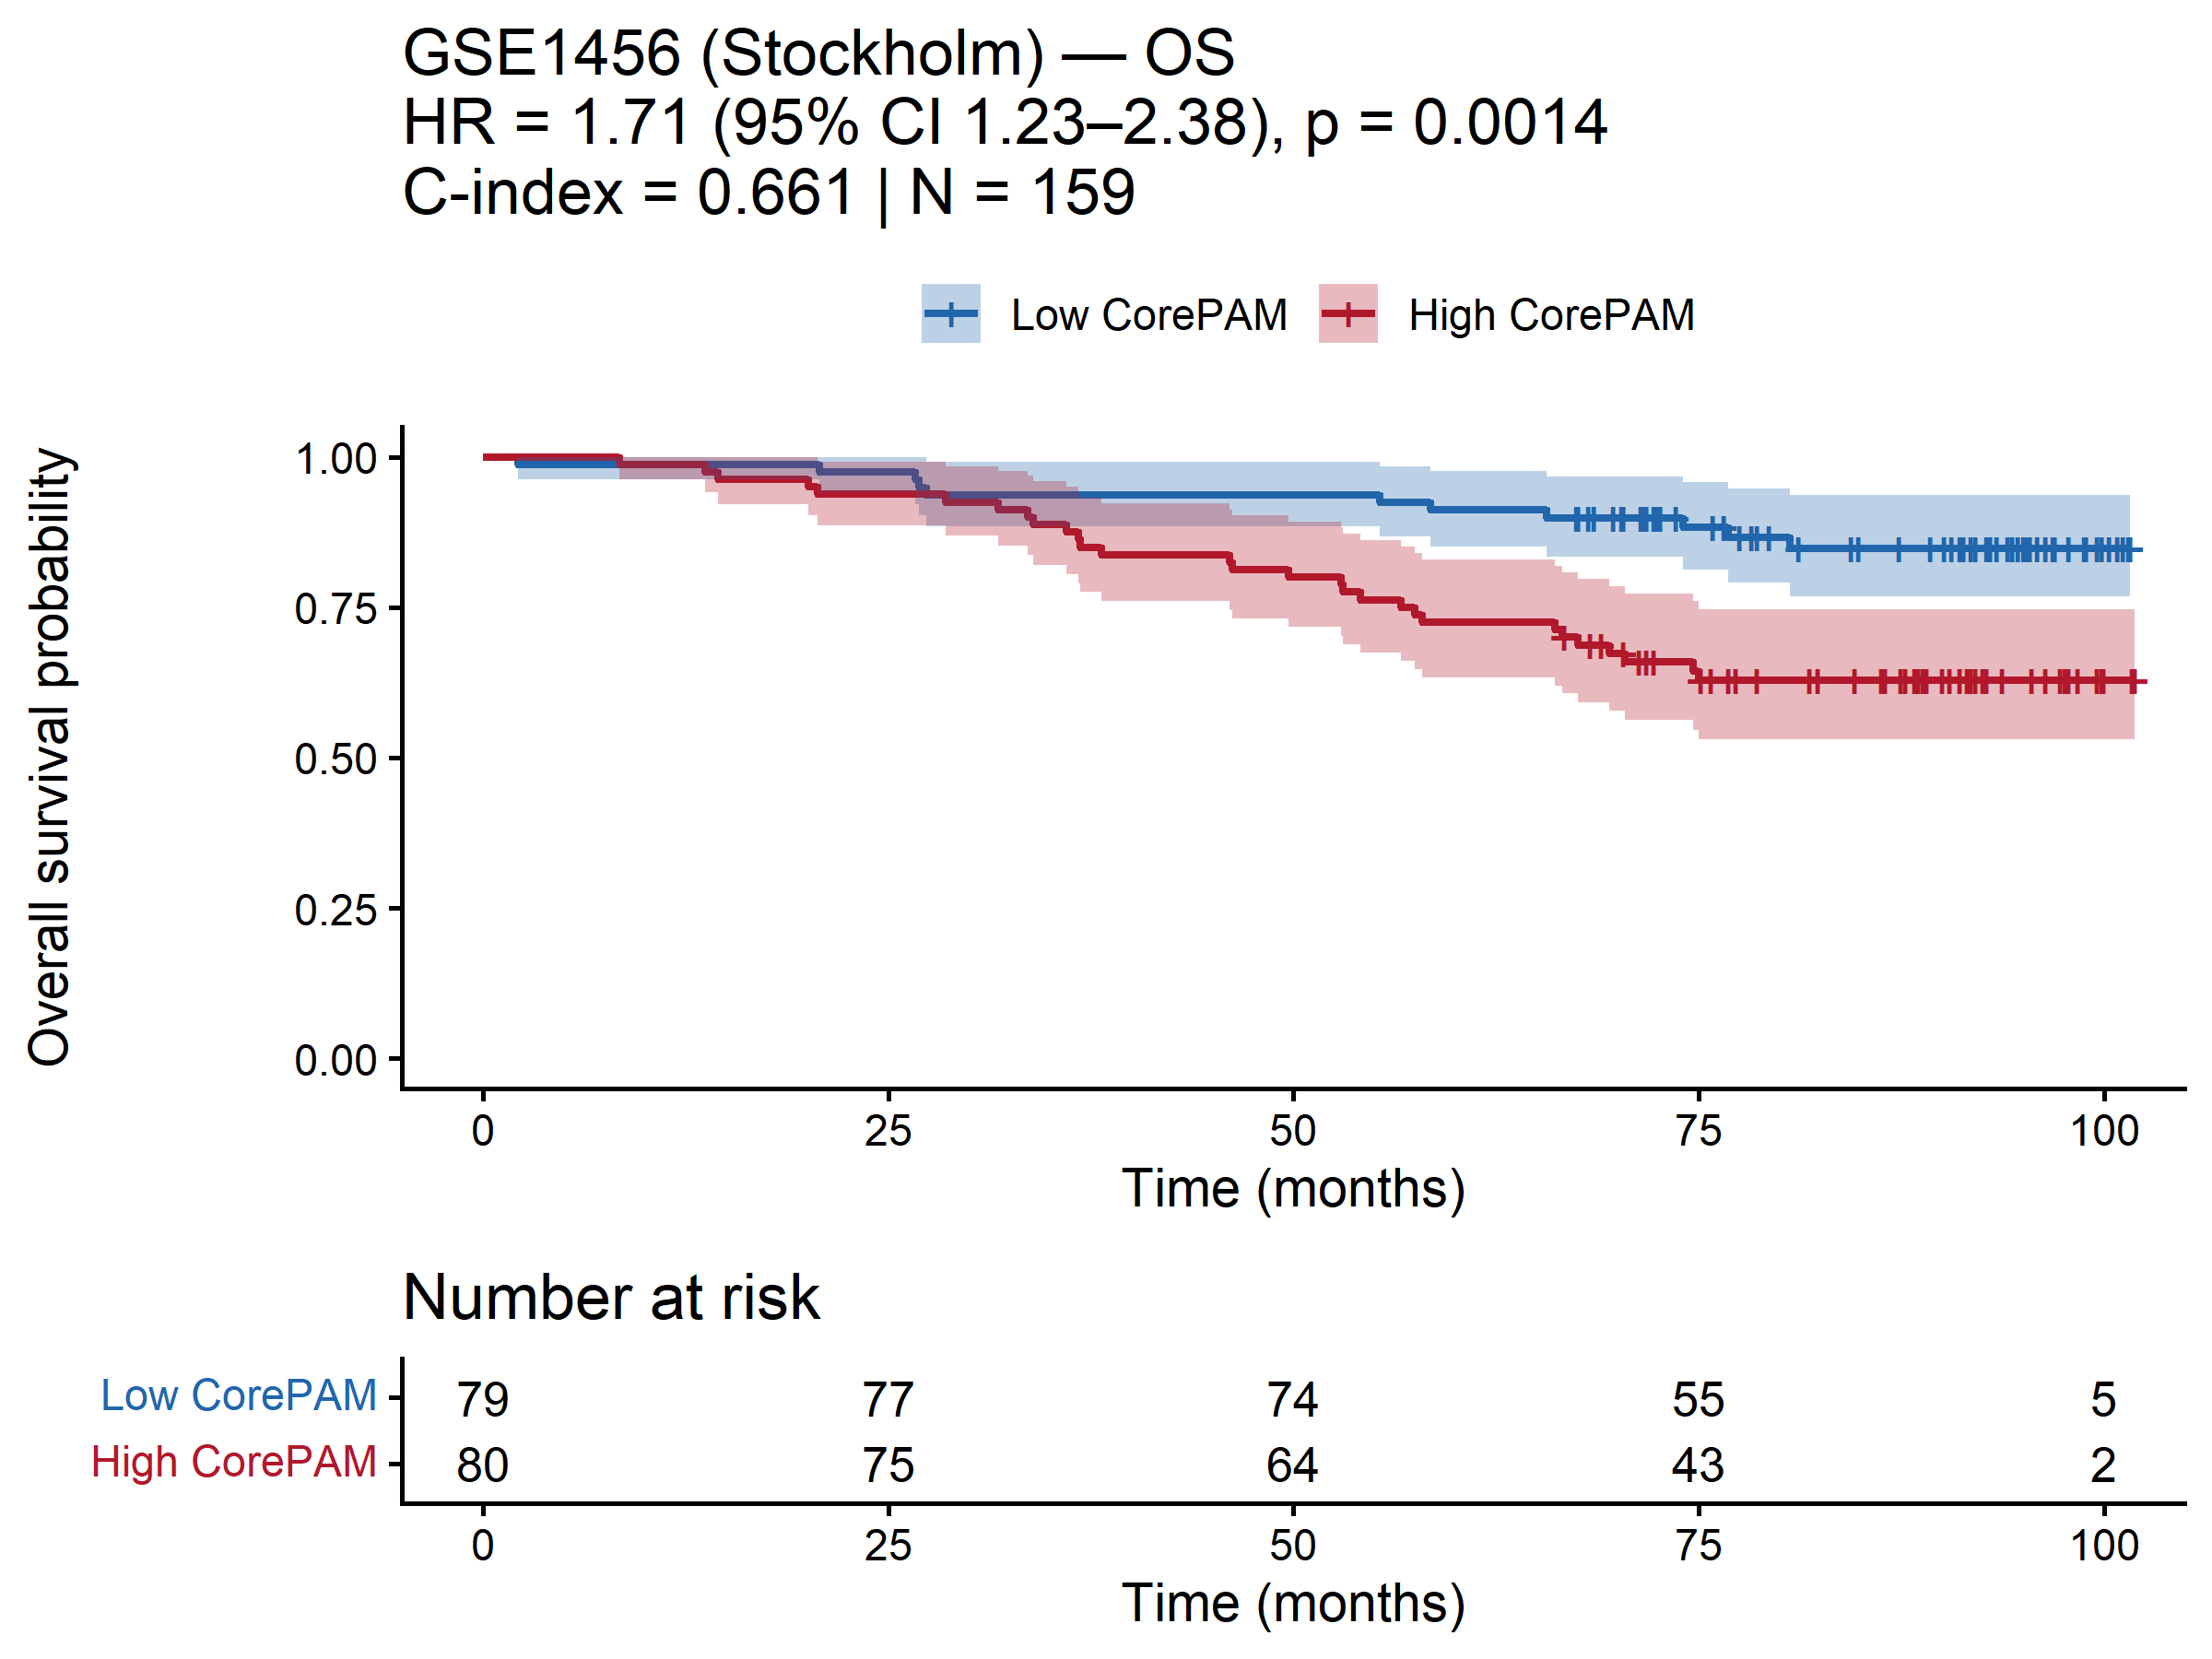
\includegraphics[width=\textwidth]{figures/Fig2_KM_GSE1456_OS_EN.png}
\caption{Kaplan--Meier overall survival curve in GSE1456 (Stockholm cohort; N = 159; 40 events; Affymetrix microarray). Patients dichotomised at the intra-cohort median CorePAM score (High vs Low). Cox HR for the dichotomised groups with 95\% CI and Wald $p$-value annotated. Shading: 95\% CI.}\label{fig:km-gse1456}
\end{figure}

TCGA-BRCA has shorter follow-up (median 32 months), attenuating the HR; a 24-month sensitivity analysis yielded HR = 1.64 (95\% CI 1.24--2.16; $p = 4.7 \times 10^{-4}$; Additional file~6: Figure~S6).

Multivariate Cox regression including the CORE-A clinical model (age and ER status where available) yielded adjusted HRs of 1.27 (TCGA-BRCA), 1.36 (METABRIC), and 1.40 (GSE20685), indicating that CorePAM provides prognostic information independent of clinical covariates. GSE1456 lacked clinical covariates for CORE-A adjustment; the univariate HR of 1.71 nonetheless confirms cross-platform generalizability on an independent Affymetrix dataset. The training cohort Kaplan--Meier curve is shown in Figure~\ref{fig:km-scanb} (in-sample C-index = 0.698; OOF C-index = 0.670).

\begin{figure}[h]
\centering
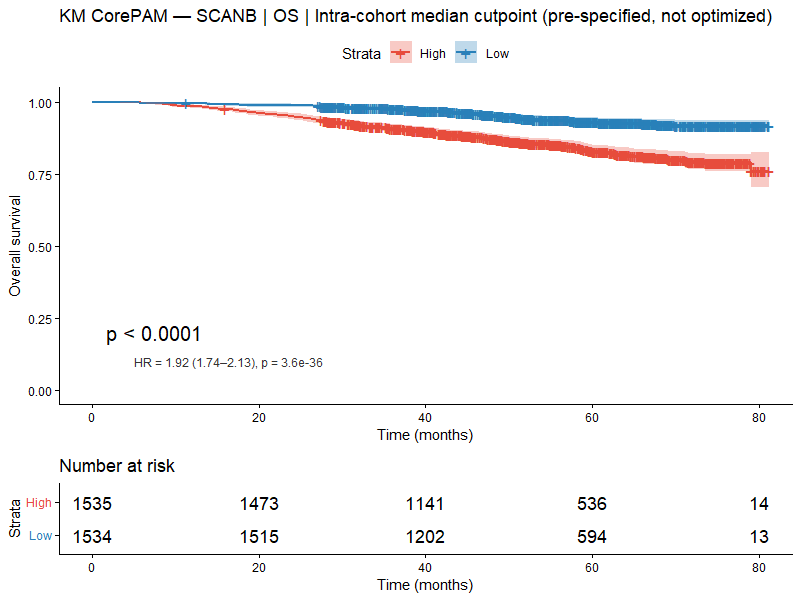
\includegraphics[width=\textwidth]{figures/Fig3_KM_SCANB_OS_CorePAM.png}
\caption{Kaplan--Meier overall survival curve in the SCAN-B training cohort (N = 3,069; 322 events; RNA-seq). Patients dichotomised at the intra-cohort median CorePAM score (High vs Low). Cox HR for the dichotomised groups with 95\% CI and Wald $p$-value annotated. Shading: 95\% CI.}\label{fig:km-scanb}
\end{figure}

\subsection{Meta-analysis}\label{subsec:results-meta}

Random-effects meta-analysis across four validation cohorts yielded a pooled HR of 1.37 (95\% CI 1.24--1.52; $p = 1.8 \times 10^{-9}$) with moderate heterogeneity ($I^2$ = 38.3\%; Figure~\ref{fig:forest-os}). The Hartung--Knapp sensitivity analysis confirmed significance under conservative inference (Table~\ref{tab:meta}). OS-harmonised and leave-one-out sensitivity analyses maintained consistent positive direction.

\begin{figure}[h]
\centering

\includegraphics[width=\textwidth]{figures/Fig4_Meta_Forest_HR_per1SD_CorePAM.png}
\caption{Forest plot of random-effects meta-analysis. HR per 1~SD CorePAM score across four validation cohorts plus pooled RE estimate (K = 4; REML estimator).}\label{fig:forest-os}
\end{figure}

\begin{table}[h]
\caption{Random-effects meta-analysis of CorePAM prognostic association (K = 4 validation cohorts).}\label{tab:meta}
\begin{tabular}{@{}llcr@{}}
\toprule
Analysis & HR (95\% CI) & $p$ & $I^2$ \\
\midrule
Primary RE (REML) & 1.37 (1.24--1.52) & $1.8 \times 10^{-9}$ & 38.3\% \\
Hartung--Knapp & 1.37 (1.15--1.64) & 0.011 & 38.3\% \\
OS-harmonised & 1.36 (1.13--1.64) & $<$0.001 & 50.5\% \\
\botrule
\end{tabular}
\end{table}

\subsection{Incremental value beyond clinical predictors}\label{subsec:results-incremental}

The CorePAM score improved the C-index over the CORE-A clinical model in all four cohorts (Table~\ref{tab:incremental}). CORE-A covariates were: age and ER status in SCAN-B and METABRIC; age alone in TCGA-BRCA and GSE20685 (where ER status was absent from harmonised clinical files). The largest increment was observed in GSE20685 ($\Delta$C = +0.093), consistent with the long follow-up and high event rate in that cohort (Figure~\ref{fig:delta-c}). Calibration at clinically relevant horizons showed adequate concordance between predicted and observed event rates in the training cohort, with expected under-confidence in external validation cohorts (Figure~\ref{fig:calibration}). Decision curve analysis confirmed net clinical benefit across a range of probability thresholds in all cohorts (Additional file~7: Figure~S7). Sensitivity analysis comparing age-only versus age + ER baselines confirmed that the CorePAM HR remains significant under both definitions (Additional file~10: Figure~S10).

\begin{table}[h]
\caption{Incremental C-index of CorePAM score over the CORE-A clinical model.}\label{tab:incremental}
\begin{tabular}{@{}llcrrl@{}}
\toprule
Cohort & CORE-A covariates & N & C (CORE-A) & C (CORE-A + CorePAM) & $\Delta$C (95\% CI) \\
\midrule
SCAN-B & age + ER & 3,069 & 0.750 & 0.780 & +0.030 (0.014--0.049) \\
TCGA-BRCA & age & 1,072 & 0.638 & 0.676 & +0.038 (0.011--0.086) \\
METABRIC & age + ER & 1,978 & 0.603 & 0.646 & +0.043 (0.025--0.066) \\
GSE20685 & age & 327 & 0.536 & 0.628 & +0.093 (0.021--0.175) \\
\botrule
\end{tabular}
\end{table}

\begin{figure}[h]
\centering

\includegraphics[width=\textwidth]{figures/Fig5_DeltaCindex_COREA_vs_COREAplus_CorePAM.png}
\caption{Incremental C-index ($\Delta$C) of CorePAM score added to the CORE-A clinical model (age $\pm$ ER status) across five cohorts. Error bars: 95\% bootstrap CI (B = 1,000). CORE-A covariates: age + ER (SCAN-B, METABRIC); age alone (TCGA-BRCA, GSE20685); not available (GSE1456).}\label{fig:delta-c}
\end{figure}

\begin{figure}[h]
\centering

\includegraphics[width=\textwidth]{figures/Fig5_Calibration_60m_Panels_CorePAM.png}
\caption{Calibration curves: predicted versus observed event rates at 60 months (SCAN-B, METABRIC, GSE20685) and 24 months (TCGA-BRCA). Diagonal: ideal calibration. Loess smoother with 95\% CI shading.}\label{fig:calibration}
\end{figure}

\subsection{Sensitivity analyses}\label{subsec:results-sensitivity}

\textbf{Frozen z-score (single-sample scoring feasibility).} When the SCAN-B training cohort mean and standard deviation per gene were frozen and applied to external validation cohorts---without any cohort-level re-standardisation---the C-index was preserved in RNA-seq and array cohorts sharing a similar dynamic range: TCGA-BRCA $\Delta$C = +0.0002 (Pearson $r$ = 0.999); METABRIC $\Delta$C = +0.0007 ($r$ = 0.958). In GSE20685, an Affymetrix U133 Plus~2 cohort with a markedly different intensity distribution, discrimination was attenuated ($\Delta$C = $-$0.042; $r$ = 0.921; frozen HR = 1.61, 95\% CI 0.87--2.96, $p$ = 0.13). The consistent preservation in RNA-seq and partial degradation in smaller microarray cohorts confirm that frozen single-sample scoring is feasible provided the assay platform is compatible with the training reference (Additional file~14: Table~S4).

\textbf{Uno's C-statistic and time-dependent AUC.} IPCW-based discrimination metrics confirmed the Harrell's C-index findings: Uno's C ranged from 0.663 (GSE20685) to 0.681 (METABRIC); time-dependent AUC at the cohort-specific horizon ranged from 0.671 (GSE20685, 60m) to 0.695 (METABRIC, 60m). These concordance estimates are robust to heterogeneous censoring (Additional file~15: Table~S5).

\textbf{Formal calibration.} Logistic recalibration at the cohort-specific horizon yielded calibration slopes ranging from 0.96 (SCAN-B, near-ideal) to 2.74 (TCGA-BRCA), with corresponding intercepts of 0.56 (SCAN-B) to 5.40 (TCGA-BRCA). The training cohort showed a near-ideal calibration slope ($\beta$ = 0.96), though the non-zero intercept ($\alpha$ = 0.56) indicates moderate systematic underprediction of absolute risk. External validation cohorts showed miscalibration that was mild in METABRIC ($\beta$ = 1.77) and GSE20685 ($\beta$ = 1.58) but substantial in TCGA-BRCA ($\beta$ = 2.74), the latter consistent with its short follow-up and low event rate at the 24-month horizon (Additional file~16: Table~S6).

\textbf{ER-stratified subgroup analysis.} In SCAN-B (N = 2,870; OS), CorePAM was significantly associated with survival in both ER-positive (HR = 1.92; 95\% CI 1.69--2.17; $p < 0.001$; N = 2,646) and ER-negative (HR = 2.53; 95\% CI 1.51--4.25; $p < 0.001$; N = 224) subgroups; the interaction test was not significant ($p$ = 0.25). In METABRIC (N = 1,936; DSS), CorePAM was strongly prognostic in ER-positive patients (HR = 1.59; 95\% CI 1.44--1.76; $p < 0.001$; N = 1,497) but showed no signal in ER-negative patients (HR = 0.97; 95\% CI 0.82--1.15; $p$ = 0.75; N = 439); the interaction was significant ($p = 3.2 \times 10^{-7}$). The discrepancy in ER-negative results reflects statistical power: SCAN-B ER$-$ had only 35 events in 224 patients (bootstrap 95\% CI for HR: 1.45--4.89; width = 3.44), whereas METABRIC ER$-$ had 186 events in 439 patients (bootstrap 95\% CI: 0.83--1.15; width = 0.32; 10.8$\times$ narrower). The well-powered METABRIC estimate indicates that the clinically meaningful signal is concentrated in ER-positive disease, consistent with the luminal biology of the retained CorePAM genes.

\subsection{Independence from clinical-pathological staging}\label{subsec:results-staging}

To address whether CorePAM retains prognostic value after adjustment for standard clinical-pathological variables, we fitted expanded multivariable Cox models adjusting for age, ER status (where available), pathological T-stage, and nodal status. T-stage and nodal status were available in 96--100\% of samples across the four cohorts with clinical covariates (SCAN-B, TCGA-BRCA, METABRIC, GSE20685). CorePAM remained independently significant in all four (all $p < 0.002$; Additional file~12: Table~S2), with HR change of less than 10\% compared to the primary CORE-A baseline. Adding CorePAM to the expanded clinical model increased the C-index by +0.022 to +0.027.

In a comprehensive secondary analysis including all six standard clinical-pathological variables (age, ER status, T-stage, nodal status, histological grade, and HER2 status), CorePAM retained independent significance in both SCAN-B (adjusted HR = 1.75; 95\% CI 1.51--2.03; $p = 1.6 \times 10^{-13}$; $\Delta$C = +0.017) and METABRIC (adjusted HR = 1.25; 95\% CI 1.14--1.38; $p = 5.5 \times 10^{-6}$; $\Delta$C = +0.015). Likelihood ratio tests confirmed that CorePAM adds significant information beyond the full clinical model (both $p < 10^{-5}$). In ER-positive patients, the incremental value was most pronounced in METABRIC ($\Delta$C = +0.032; 95\% CI 0.018--0.050; LRT $p = 10^{-10}$).

\subsection{Pathologic complete response (secondary analysis)}\label{subsec:results-pcr}

In four independent neoadjuvant cohorts (N = 697 total), the CorePAM score showed a positive association with pCR in all four cohorts, reaching statistical significance in three of four (Table~\ref{tab:pcr}). GSE25066 showed a positive but non-significant trend (OR = 1.44; $p = 0.060$). ORs ranged from 1.44 to 2.10 per 1~SD. The AUC ranged from 0.576 to 0.716, indicating moderate to good discriminative ability for pCR prediction.

\begin{table}[h]
\caption{CorePAM score predicts pCR in neoadjuvant chemotherapy cohorts.}\label{tab:pcr}
\begin{tabular}{@{}lrlllcl@{}}
\toprule
Cohort & N & pCR, n (\%) & OR per 1~SD (95\% CI) & $p$ & AUC (95\% CI) \\
\midrule
GSE25066 & 182 & 42 (23.1\%) & 1.44 (0.98--2.09) & 0.060 & 0.576 (0.477--0.676) \\
GSE20194 & 278 & 56 (20.1\%) & 1.73 (1.25--2.38) & $<$0.001 & 0.660 (0.586--0.734) \\
GSE32646 & 115 & 27 (23.5\%) & 2.10 (1.31--3.39) & 0.002 & 0.716 (0.611--0.821) \\
I-SPY1 & 122 & 32 (26.2\%) & 1.66 (1.05--2.63) & 0.030 & 0.622 (0.517--0.726) \\
\midrule
\textbf{RE pooled} & \textbf{697} & & \textbf{1.69 (1.39--2.05)} & $\mathbf{<}$\textbf{0.001} & \\
\botrule
\end{tabular}
\footnotetext{OR: odds ratio per 1~SD CorePAM score; AUC: area under the receiver operating characteristic curve; RE: random effects (DerSimonian--Laird). $I^2$ = 0\%.}
\end{table}

Random-effects meta-analysis yielded a pooled OR of 1.69 (95\% CI 1.39--2.05; $I^2$ = 0\%; $p = 1.9 \times 10^{-7}$; Figure~\ref{fig:forest-pcr}). The absence of heterogeneity across four cohorts from different platforms and trials reinforces the cross-platform consistency of the CorePAM pCR association.

\begin{figure}[h]
\centering
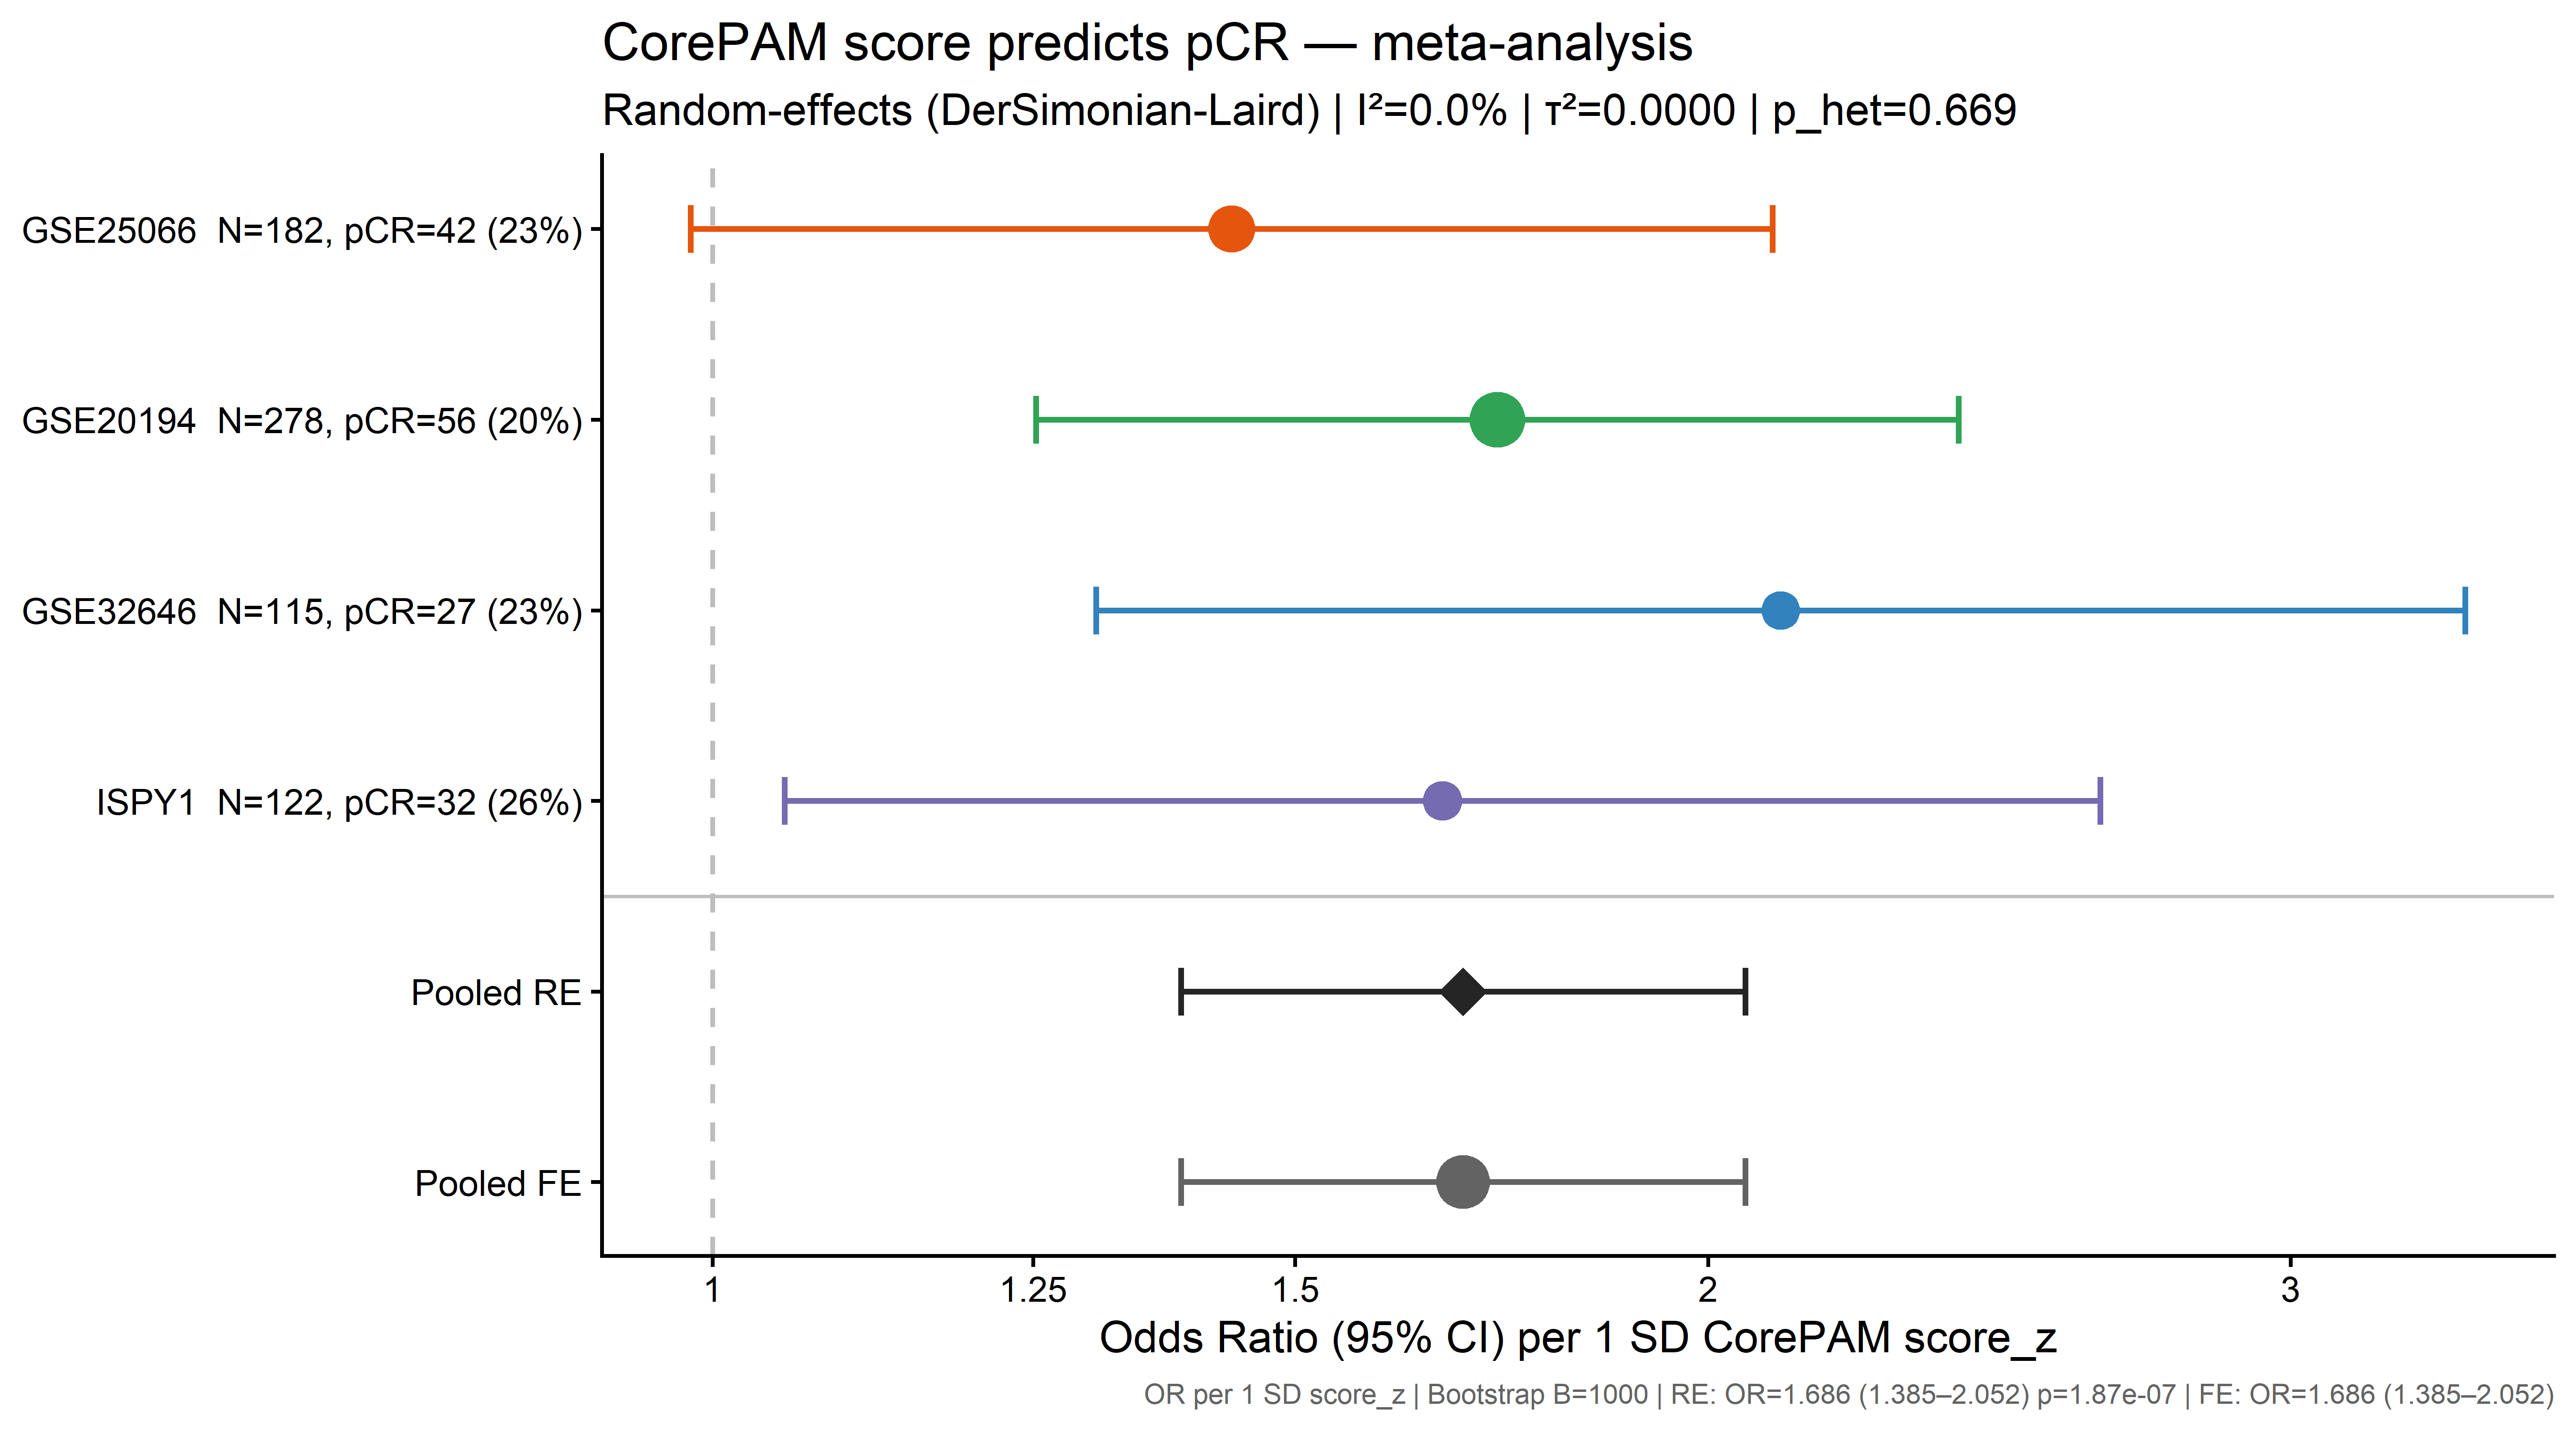
\includegraphics[width=\textwidth]{figures/Fig_pCR1_Forest_OR_EN.png}
\caption{Forest plot of CorePAM and pathologic complete response (pCR). OR per 1~SD CorePAM score (univariate logistic regression) in four independent neoadjuvant chemotherapy cohorts (GSE25066, GSE20194, GSE32646, I-SPY1; total N = 697), with random-effects pooled estimate (DerSimonian--Laird; $I^2$ = 0\%).}\label{fig:forest-pcr}
\end{figure}

\textbf{I-SPY2 exploratory analysis.} In the I-SPY2 external exploratory cohort (GSE194040; N = 986; pCR rate = 32.4\%), the CorePAM score predicted pCR univariately (OR = 1.68; 95\% CI 1.45--1.95; AUC = 0.648). Inclusion of I-SPY2 in the meta-analysis ($k = 5$) yielded OR = 1.69 (95\% CI 1.50--1.90; $I^2$ = 0\%), virtually identical to the primary analysis, confirming external generalizability.

%% ============================================================
%%  DISCUSSION
%% ============================================================
\section{Discussion}\label{sec:discussion}

We demonstrate that CorePAM---a 24-gene data-driven reduction of the PAM50 panel---achieves non-inferior prognostic performance relative to a full 50-gene Cox elastic-net model in four independent external cohorts spanning RNA-seq and microarray platforms. The comparator is a 50-gene Cox elastic-net model, not the commercial Prosigna/PAM50 assay (which uses centroid-based subtyping plus ROR); the non-inferiority claim is scoped to this elastic-net framework. No claims of therapeutic equivalence or clinical decision-making impact are made.

\textbf{Reproducible derivation.} Fold assignment was deterministic (SHA-256 of patient identifiers), eliminating random seeds as a driver of gene selection and ensuring exact reproducibility from first principles. The gene count (N = 24) was not pre-specified; it was derived from the Pareto frontier of model complexity versus OOF C-index (Additional file~1: Figure~S1), where performance plateaus well before 50 genes.

\textbf{Gene selection stability.} Bootstrap resampling ($B = 200$ refits on SCAN-B) confirmed that 15 of 24 CorePAM genes were selected in at least 70\% of resamples (Additional file~8: Figure~S8), with 2 genes (ACTR3B, NAT1) selected in 100\%. The remaining genes show lower but non-negligible selection frequencies (minimum: 35.5\%), consistent with the elastic-net grouping property that distributes weight among correlated genes. Leave-one-gene-out analysis showed that no single gene removal causes catastrophic performance loss (Additional file~9: Figure~S9; maximum $|\Delta C|$ = 0.044).

\textbf{Heterogeneity is expected and informative.} The moderate $I^2$ in the OS/DSS meta-analysis reflects two structural sources: endpoint divergence (DSS in METABRIC vs.\ OS in the other cohorts) and differential follow-up duration (32 months in TCGA-BRCA vs.\ 91--159 months elsewhere). The OS-harmonised sensitivity analysis (substituting METABRIC OS for DSS) reduced $I^2$ substantially, confirming the pooled estimate is not driven by endpoint choice. The key finding is the consistency of \textit{direction}---a positive HR in all four validation cohorts---rather than effect magnitude. The Hartung--Knapp sensitivity analysis confirmed significance under conservative inference.

\textbf{Biological coherence.} The retained genes recapitulate core PAM50 biology: luminal differentiation (ESR1, PGR, BCL2, NAT1), proliferation (MYBL2, PTTG1, EXO1, MYC), basal phenotype (KRT5, KRT17, FOXC1), and HER2-enriched markers (ERBB2, GRB7). The proliferation genes also explain the pCR signal, as these pathways are targeted by anthracycline-taxane regimens. The 26 excluded genes received zero weight at the selected $\lambda$, consistent with functional redundancy under the elastic-net grouping property.

\textbf{Cross-platform consistency in pCR prediction.} The pCR block showed no heterogeneity ($I^2$ = 0\% across four cohorts), consistent with the biological basis of the signal: the retained proliferation genes are directly targeted by standard neoadjuvant regimens~\cite{prat2015}.

\textbf{Calibration and clinical utility.} Calibration at clinically relevant horizons (60 months for SCAN-B, METABRIC, GSE20685; 24 months for TCGA-BRCA) showed adequate concordance between predicted and observed event rates in the training cohort (Figure~\ref{fig:calibration}). Formal logistic recalibration confirmed a near-ideal calibration slope in the training cohort ($\beta$ = 0.96; intercept $\alpha$ = 0.56, indicating moderate underprediction of absolute risk) with further miscalibration in external cohorts (slopes 1.58--2.74), consistent with model under-confidence when applying scores cross-platform without recalibration---a structural property of intra-cohort z-scoring. Decision curve analysis confirmed positive net benefit across a range of probability thresholds in all cohorts (Additional file~7: Figure~S7).

\textbf{Frozen z-score supports clinical translation.} A key reviewer concern was whether the intra-cohort z-score normalisation---appropriate for retrospective multi-cohort validation---could support single-sample scoring. Our frozen z-score sensitivity analysis applied SCAN-B reference mean/SD per gene to each external cohort without any cohort-level re-standardisation, ensuring that each patient's score depends only on their own expression values and the frozen reference. Discrimination was preserved in TCGA-BRCA ($\Delta$C = +0.0002; $r$ = 0.999) and METABRIC ($\Delta$C = +0.0007; $r$ = 0.958). In GSE20685 (Affymetrix U133 Plus~2), frozen scoring showed measurable degradation ($\Delta$C = $-$0.042; $r$ = 0.921), consistent with the larger distributional gap between RNA-seq and this microarray platform. These results confirm that a fixed normalisation reference can support single-sample scoring when the assay platform is compatible with the training reference.

\textbf{Uno's C-statistic confirms robustness to censoring.} IPCW-based concordance metrics (Uno's C, time-dependent AUC) yielded estimates consistent with Harrell's C-index, confirming that the observed discrimination is not an artefact of heterogeneous censoring distributions across cohorts.

\textbf{ER subgroup analysis.} CorePAM is prognostic in unselected cohorts overall, with the clinically meaningful signal concentrated in ER-positive disease. In both SCAN-B and METABRIC, the ER-positive HR was robust (1.92 and 1.59, respectively; both $p < 0.001$). In ER-negative patients, SCAN-B showed an apparent effect (HR = 2.53) that was not replicated in the better-powered METABRIC analysis (HR = 0.97; N = 439, 186 events). Bootstrap analysis confirmed that the SCAN-B ER-negative estimate is highly unstable (95\% CI width = 3.44 vs 0.32 in METABRIC), consistent with its small sample (35 events). This behaviour is consistent with luminal biology and with the clinical use of multigene prognostic assays primarily in ER-positive disease~\cite{sparano2018,dowsett2013}.

\textbf{Independence from clinical-pathological staging.} CorePAM retained independent prognostic value after adjustment for all six standard clinical-pathological variables (age, ER, T-stage, N-status, grade, HER2) in both SCAN-B (LRT $p = 4.9 \times 10^{-13}$) and METABRIC (LRT $p = 6.1 \times 10^{-6}$). The $\Delta$C of +0.015 to +0.017 over this comprehensive baseline---and +0.032 in ER-positive METABRIC---confirms that CorePAM captures molecular heterogeneity not accessible through routine clinical-pathological assessment.

\textbf{Comparison with established signatures.} An exploratory head-to-head comparison against research-based implementations (genefu R package~\cite{gendoo2016}) of the PAM50-derived Risk of Recurrence score (ROR-S, 50 genes) and the OncotypeDX Recurrence Score (ODX-RS, 21 genes) showed that CorePAM (24 genes) performs competitively (Additional file~13: Table~S3). CorePAM showed advantages in the RNA-seq cohorts (its training domain) and small deficits ($\Delta$C $< 0.03$) in the microarray cohorts (the development domain of those signatures). This comparison involves research-based score implementations---not commercial assays---and should be interpreted as evidence of competitive performance, not clinical equivalence.

\textbf{Clinical implications.} A 24-gene panel can be measured by a variety of RT-PCR, NanoString nCounter, or targeted RNA-seq platforms that are unable to reliably quantify all 50 PAM50 genes. If validated in prospective cohorts, CorePAM could extend the reach of molecular stratification to resource-limited settings.

\textbf{Limitations.} This is a retrospective study using public data. TCGA-BRCA has structurally short follow-up (median 32 months), attenuating the detectable HR; the 24-month sensitivity analysis (Additional file~6: Figure~S6) partially mitigates this. METABRIC uses DSS as the primary endpoint, following established precedent for that dataset. Two CorePAM genes are absent from the Affymetrix HGU133A platform used in GSE20685 (22/24 = 91.7\% coverage); gene dropout sensitivity analysis confirmed minimal impact (Additional file~9: Figure~S9). The primary CORE-A clinical baseline was restricted to age and ER status---the two variables consistently available in harmonised form---although expanded models including T-stage and nodal status confirmed independent prognostic value (Additional file~12: Table~S2). ER status was unavailable in TCGA-BRCA and GSE20685, restricting CORE-A to age alone in those cohorts. Comparisons with ROR-S and ODX-RS used research-based implementations, not commercial assays. No prospective validation was performed. The primary score formulation uses intra-cohort z-score normalisation; however, a frozen z-score sensitivity analysis (using SCAN-B reference parameters without cohort-level re-standardisation) demonstrated preserved discrimination in RNA-seq and Illumina array cohorts ($\Delta$C $<$ 0.001) and honest degradation in the Affymetrix cohort ($\Delta$C = $-$0.042), supporting the feasibility of single-sample scoring with a fixed reference for compatible platforms. Full clinical translation would additionally require platform-specific housekeeping-gene calibration, which is the subject of future technical validation work. HER2 status was not available in sufficient cohorts to permit HER2-stratified subgroup analysis.

%% ============================================================
%%  CONCLUSIONS
%% ============================================================
\section{Conclusions}\label{sec:conclusions}

CorePAM is a 24-gene data-driven reduction of the PAM50 panel, derived without pre-specifying gene count, that achieves non-inferior prognostic discrimination relative to a full 50-gene Cox elastic-net model across four independent validation cohorts and two distinct expression platforms (RNA-seq and microarray). The score provides incremental value beyond a comprehensive six-variable clinical baseline (age, ER, T-stage, N-status, grade, HER2; LRT $p < 10^{-5}$), with the clinically meaningful signal concentrated in ER-positive disease. CorePAM also predicts pathologic complete response to neoadjuvant chemotherapy with high cross-cohort consistency ($I^2$ = 0\%). The analytical pipeline is fully reproducible from publicly available data.

%% ============================================================
%%  BACKMATTER
%% ============================================================
\backmatter

\section*{List of abbreviations}

\noindent
AUC: Area under the curve;
CI: Confidence interval;
CORE-A: Clinical baseline model (age $\pm$ ER status);
CPM: Counts per million;
CV: Cross-validation;
DCA: Decision curve analysis;
DL: DerSimonian--Laird;
DSS: Disease-specific survival;
ER: Estrogen receptor;
FFPE: Formalin-fixed paraffin-embedded;
GDC: Genomic Data Commons;
GEO: Gene Expression Omnibus;
HER2: Human epidermal growth factor receptor 2;
HGNC: HUGO Gene Nomenclature Committee;
HR: Hazard ratio;
KM: Kaplan--Meier;
LLM: Large language model;
OOF: Out-of-fold;
OR: Odds ratio;
OS: Overall survival;
PAM50: Prediction Analysis of Microarray 50;
PCA: Principal component analysis;
pCR: Pathologic complete response;
RE: Random effects;
REML: Restricted maximum likelihood;
ROR-S: Risk of Recurrence score (subtype-based);
SD: Standard deviation;
SE: Standard error;
TMM: Trimmed mean of M-values.

\bmhead{Supplementary information}

Additional files 1--17 are available as supplementary material. See the Additional files section at the end of this article for descriptions.

\bmhead{Acknowledgements}

The authors thank the SCAN-B, TCGA, METABRIC, I-SPY, and Stockholm (GSE1456) consortia for making their data publicly available.

\section*{Declarations}

\begin{description}
\item[Ethics approval and consent to participate] Not applicable. This study uses exclusively publicly available de-identified data (GEO, GDC, cBioPortal). No new human subjects research was conducted.
\item[Consent for publication] Not applicable.
\item[Availability of data and materials] All raw data are available through GEO (GSE96058, GSE25066, GSE20194, GSE32646, GSE22226, GSE194040, GSE1456), GDC (TCGA-BRCA), and cBioPortal (METABRIC). Analysis code, frozen analytical parameters, and a single-command reproducibility script are available at \url{https://github.com/RafaelBotan/CorePAM-Study}~\cite{botan2026} (release tagged at submission). All results can be reproduced from raw public data using the provided pipeline.
\item[Competing interests] The authors declare no competing interests.
\item[Funding] No external funding was received. This study was conducted independently by the authors.
\item[Authors' contributions] RB designed the study, performed all analyses, and wrote the manuscript. JBS supervised the study and reviewed the manuscript. Both authors read and approved the final manuscript.
\end{description}

%% ============================================================
%%  ADDITIONAL FILES
%% ============================================================
\section*{Additional files}

%% --- Figure S1 ---
\begin{figure}[p]
\centering
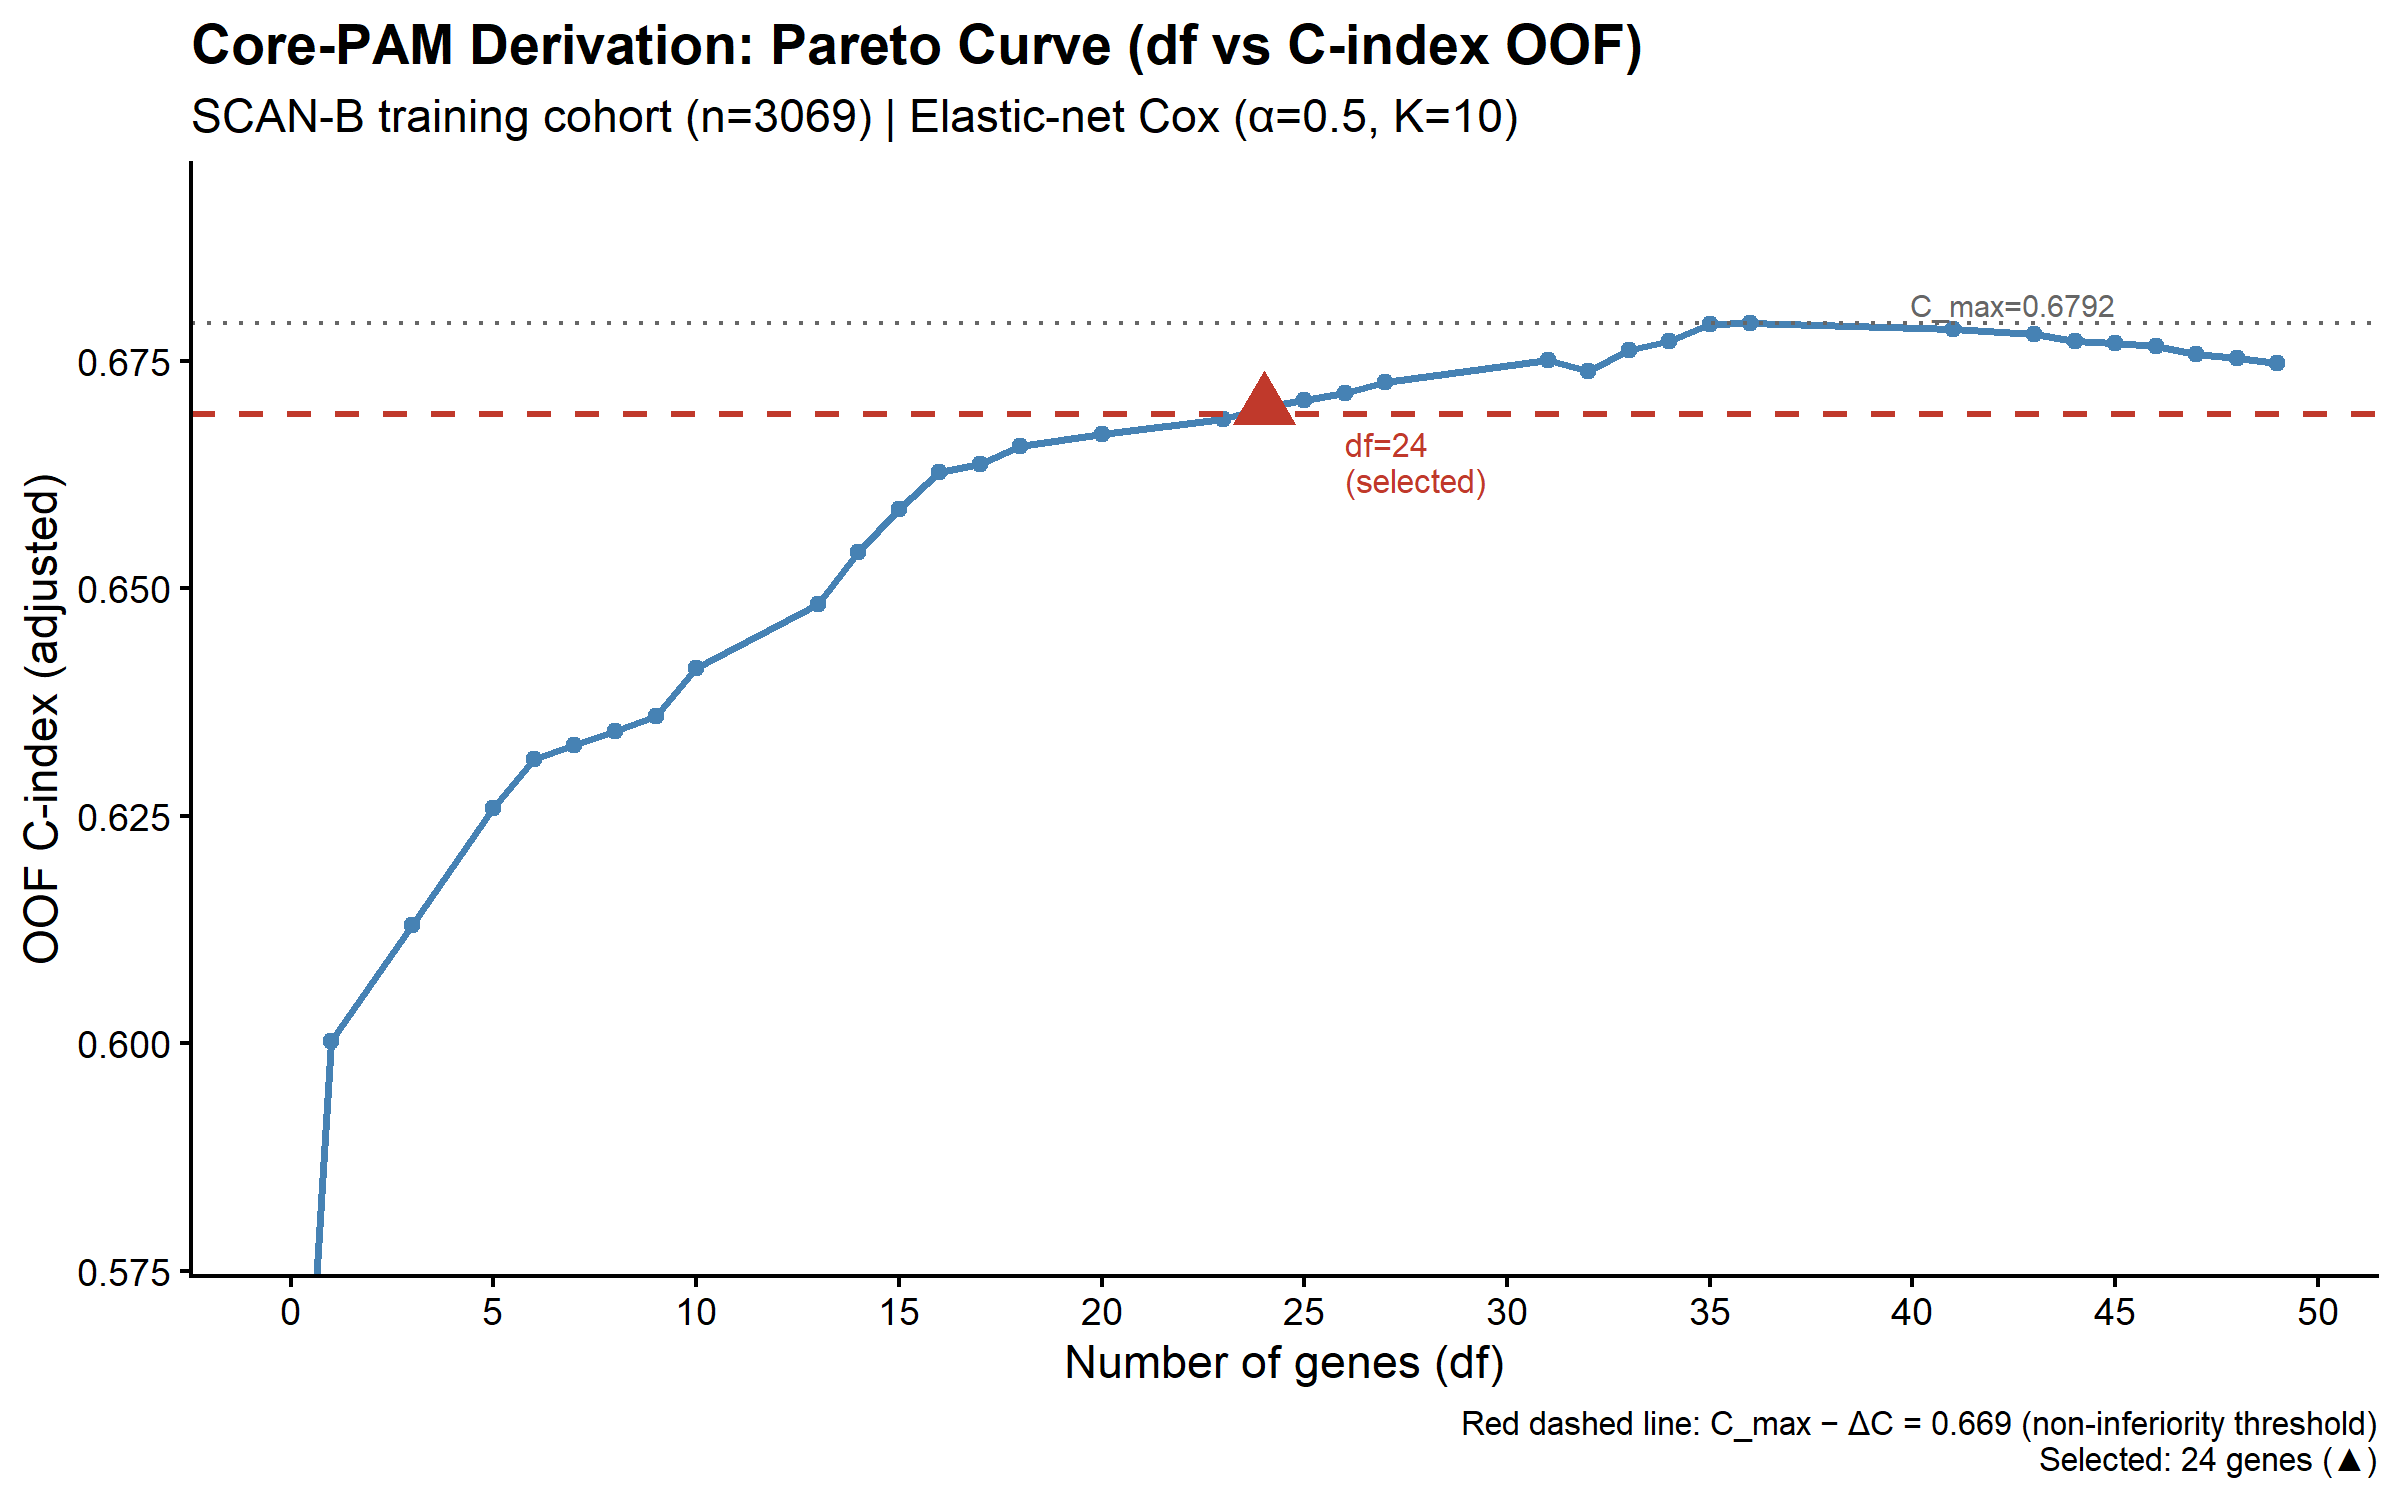
\includegraphics[width=\textwidth,height=0.85\textheight,keepaspectratio]{additional_files/Additional_file_01_FigS1_Pareto.png}
\caption{\textbf{Additional file~1: Figure~S1.} Pareto frontier: gene count vs.\ OOF C-index. Each point represents a unique df level along the glmnet regularisation path. Dashed red line: non-inferiority boundary ($C_{\text{max}} - \Delta C$; $\Delta C = 0.010$).}\label{fig:s1-pareto}
\end{figure}

%% --- Figure S2 ---
\begin{figure}[p]
\centering
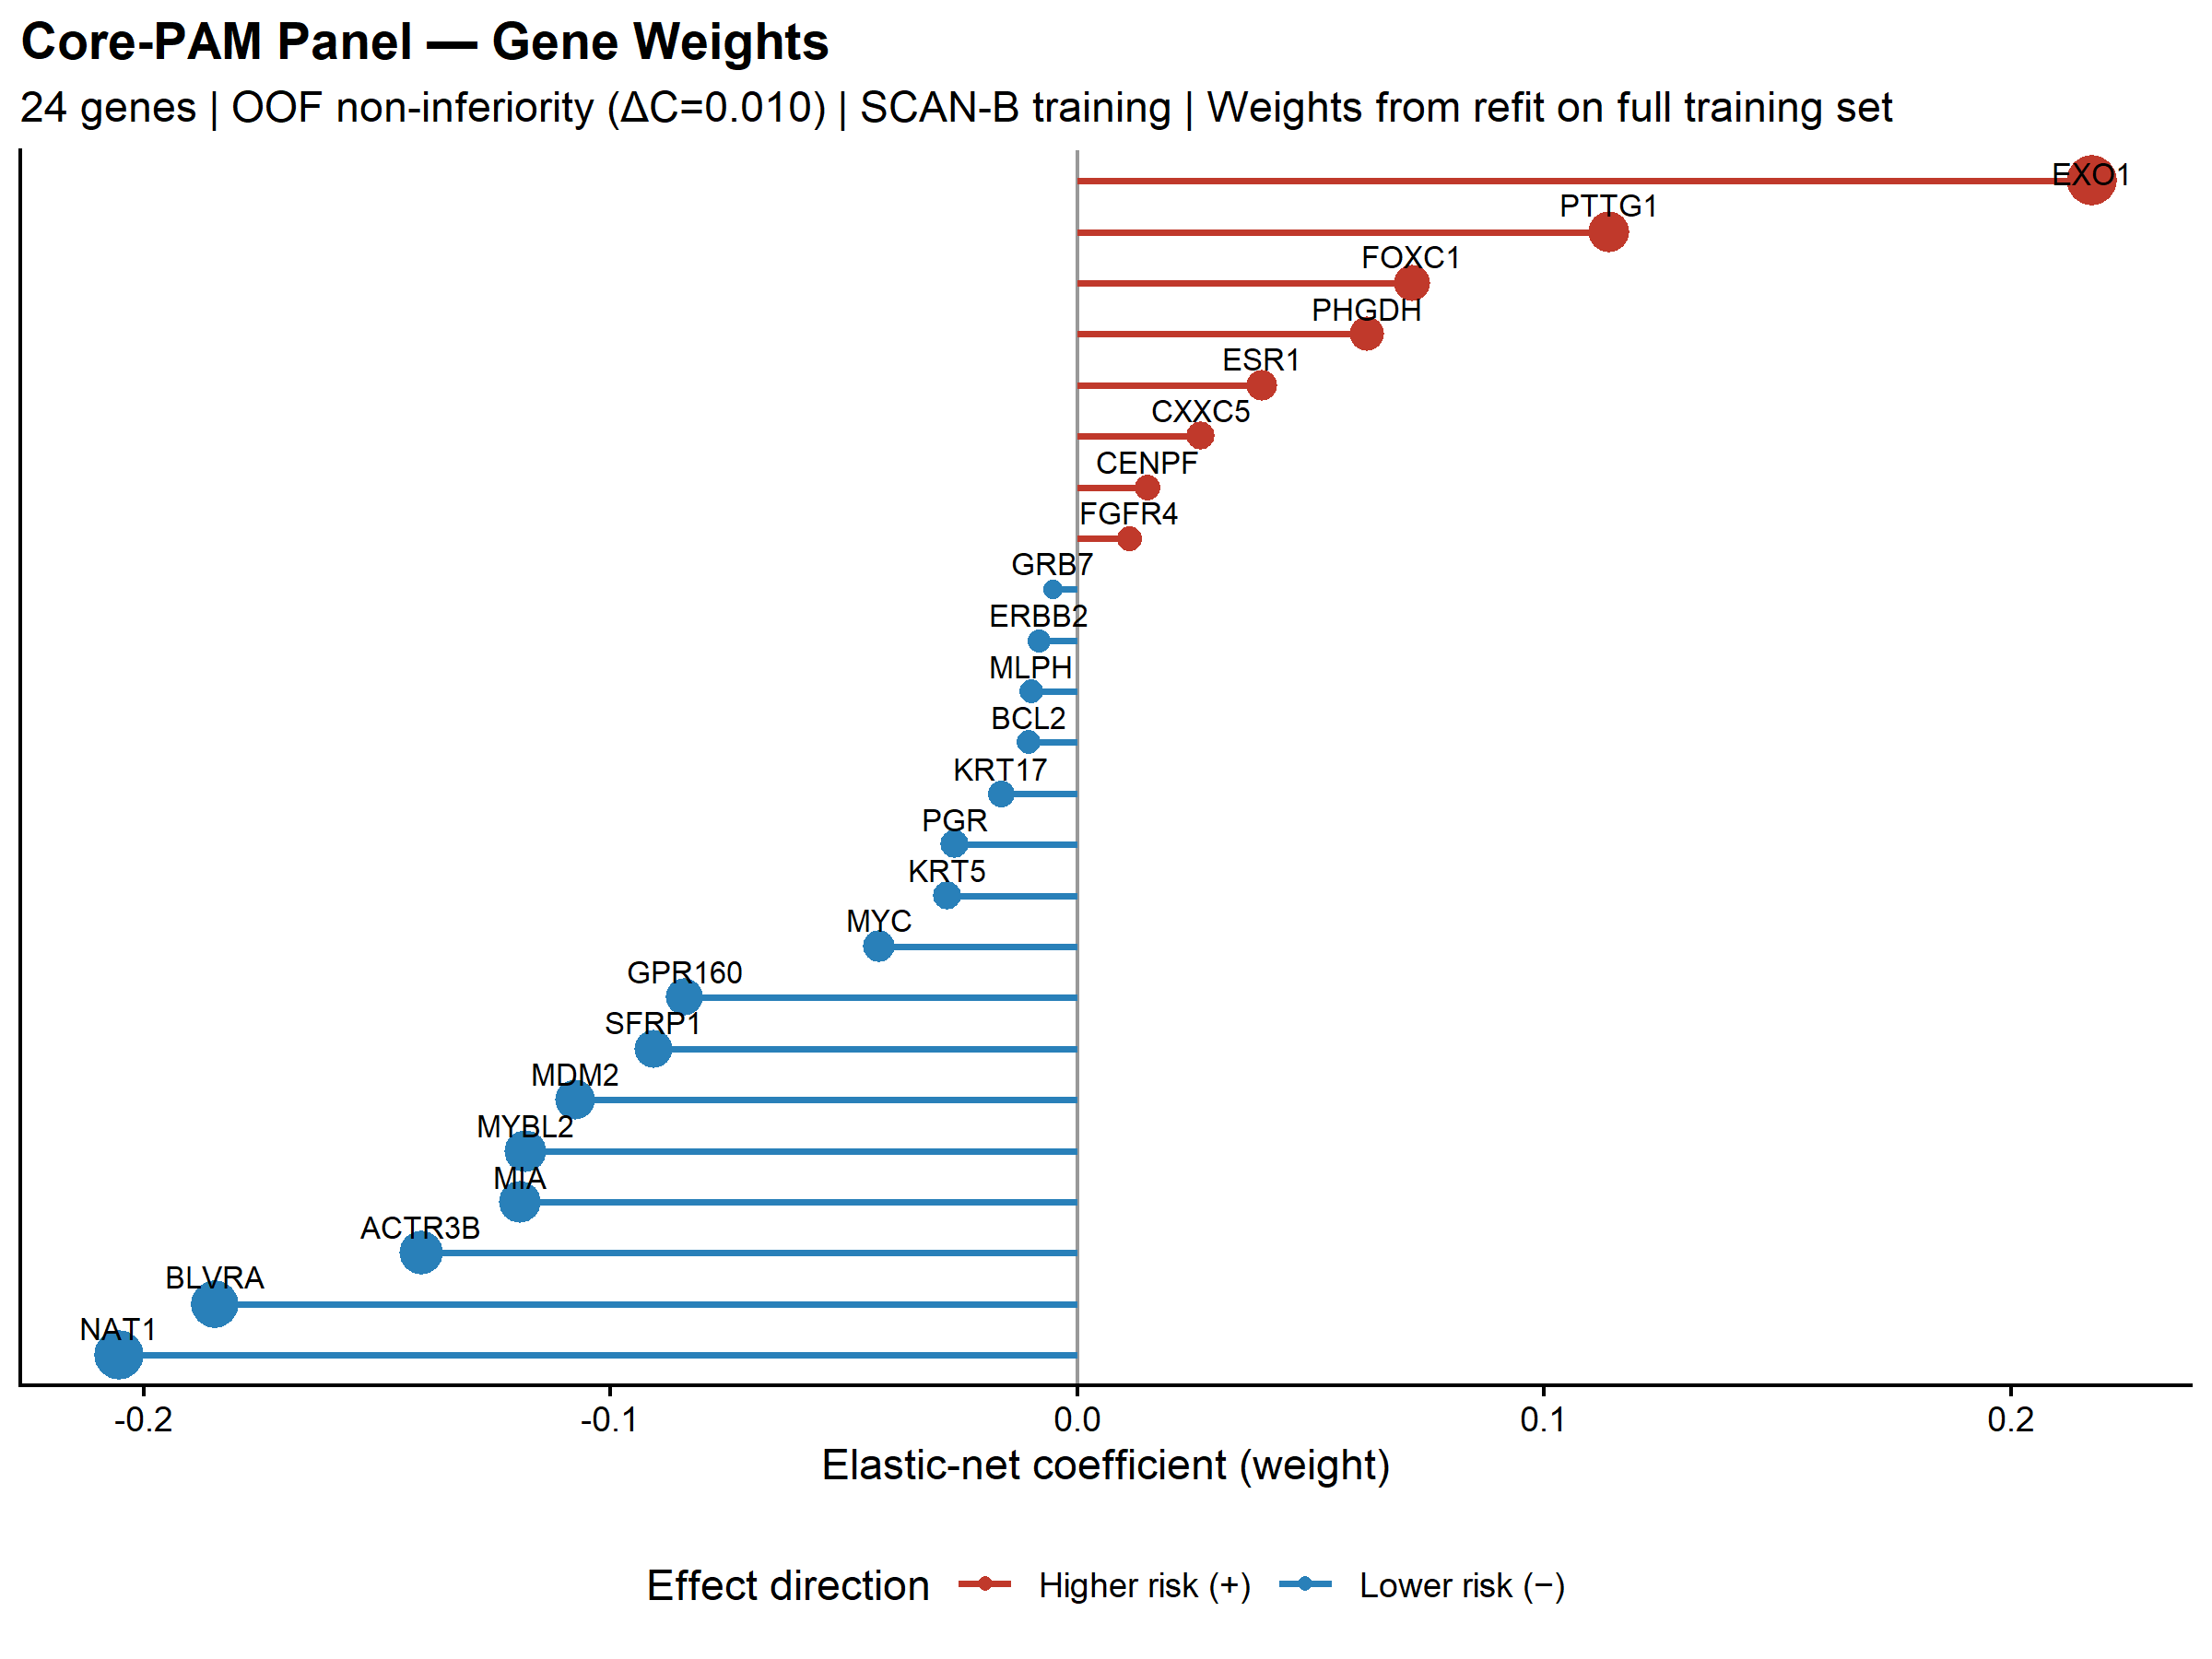
\includegraphics[width=\textwidth,height=0.85\textheight,keepaspectratio]{additional_files/Additional_file_02_FigS2_Weights.png}
\caption{\textbf{Additional file~2: Figure~S2.} CorePAM gene weights (lollipop plot). Elastic-net Cox regression coefficients. Positive weights (red): higher expression associated with worse survival.}\label{fig:s2-weights}
\end{figure}

%% --- Figure S3 ---
\begin{figure}[p]
\centering
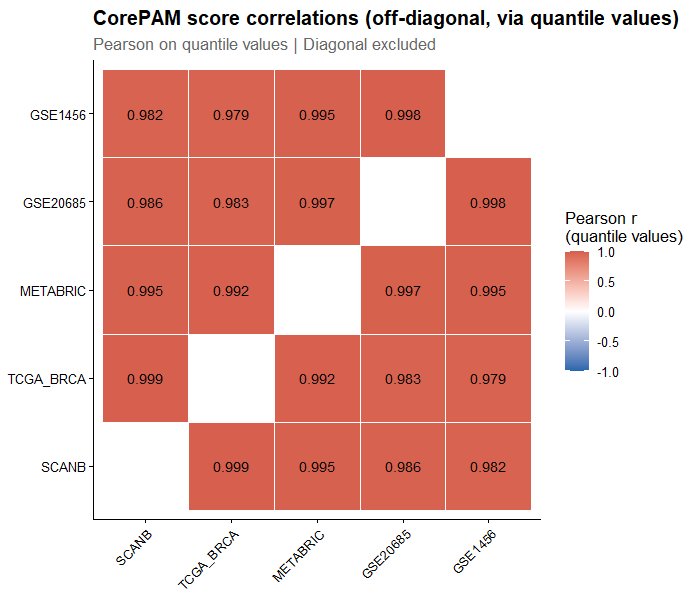
\includegraphics[width=\textwidth,height=0.85\textheight,keepaspectratio]{additional_files/Additional_file_03_FigS3_Correlation.png}
\caption{\textbf{Additional file~3: Figure~S3.} Off-diagonal CorePAM score correlations between cohorts. Pearson $r$ computed on paired quantile values.}\label{fig:s3-correlation}
\end{figure}

%% --- Figure S4 ---
\begin{figure}[p]
\centering
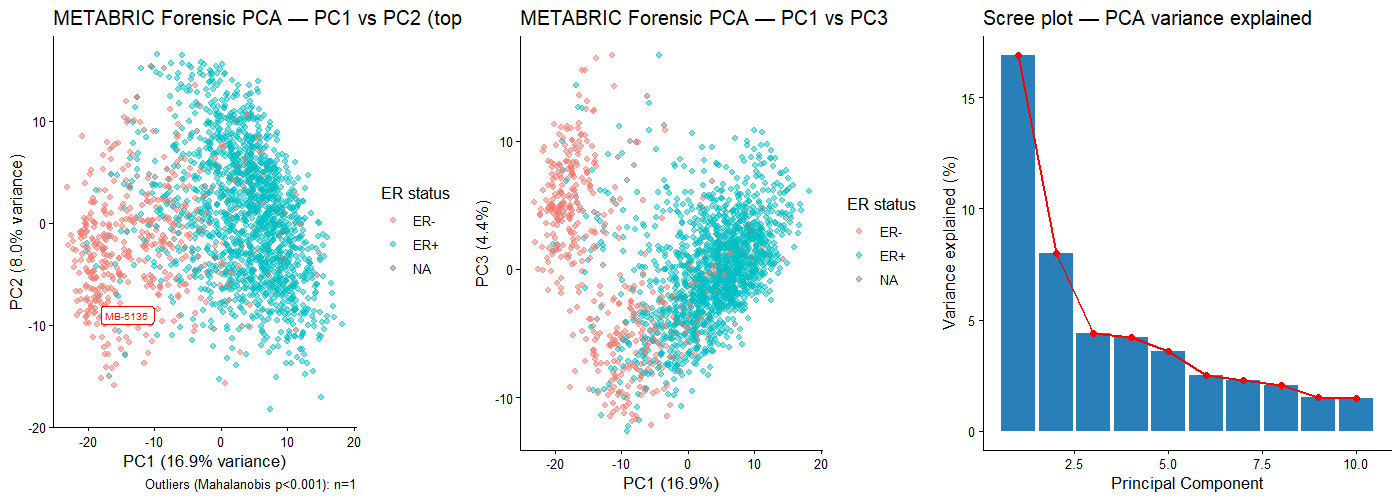
\includegraphics[width=\textwidth,height=0.85\textheight,keepaspectratio]{additional_files/Additional_file_04_FigS4_PCA.png}
\caption{\textbf{Additional file~4: Figure~S4.} Forensic PCA of METABRIC expression matrix. Principal component analysis coloured by ER status.}\label{fig:s4-pca}
\end{figure}

%% --- Figure S5 ---
\begin{figure}[p]
\centering
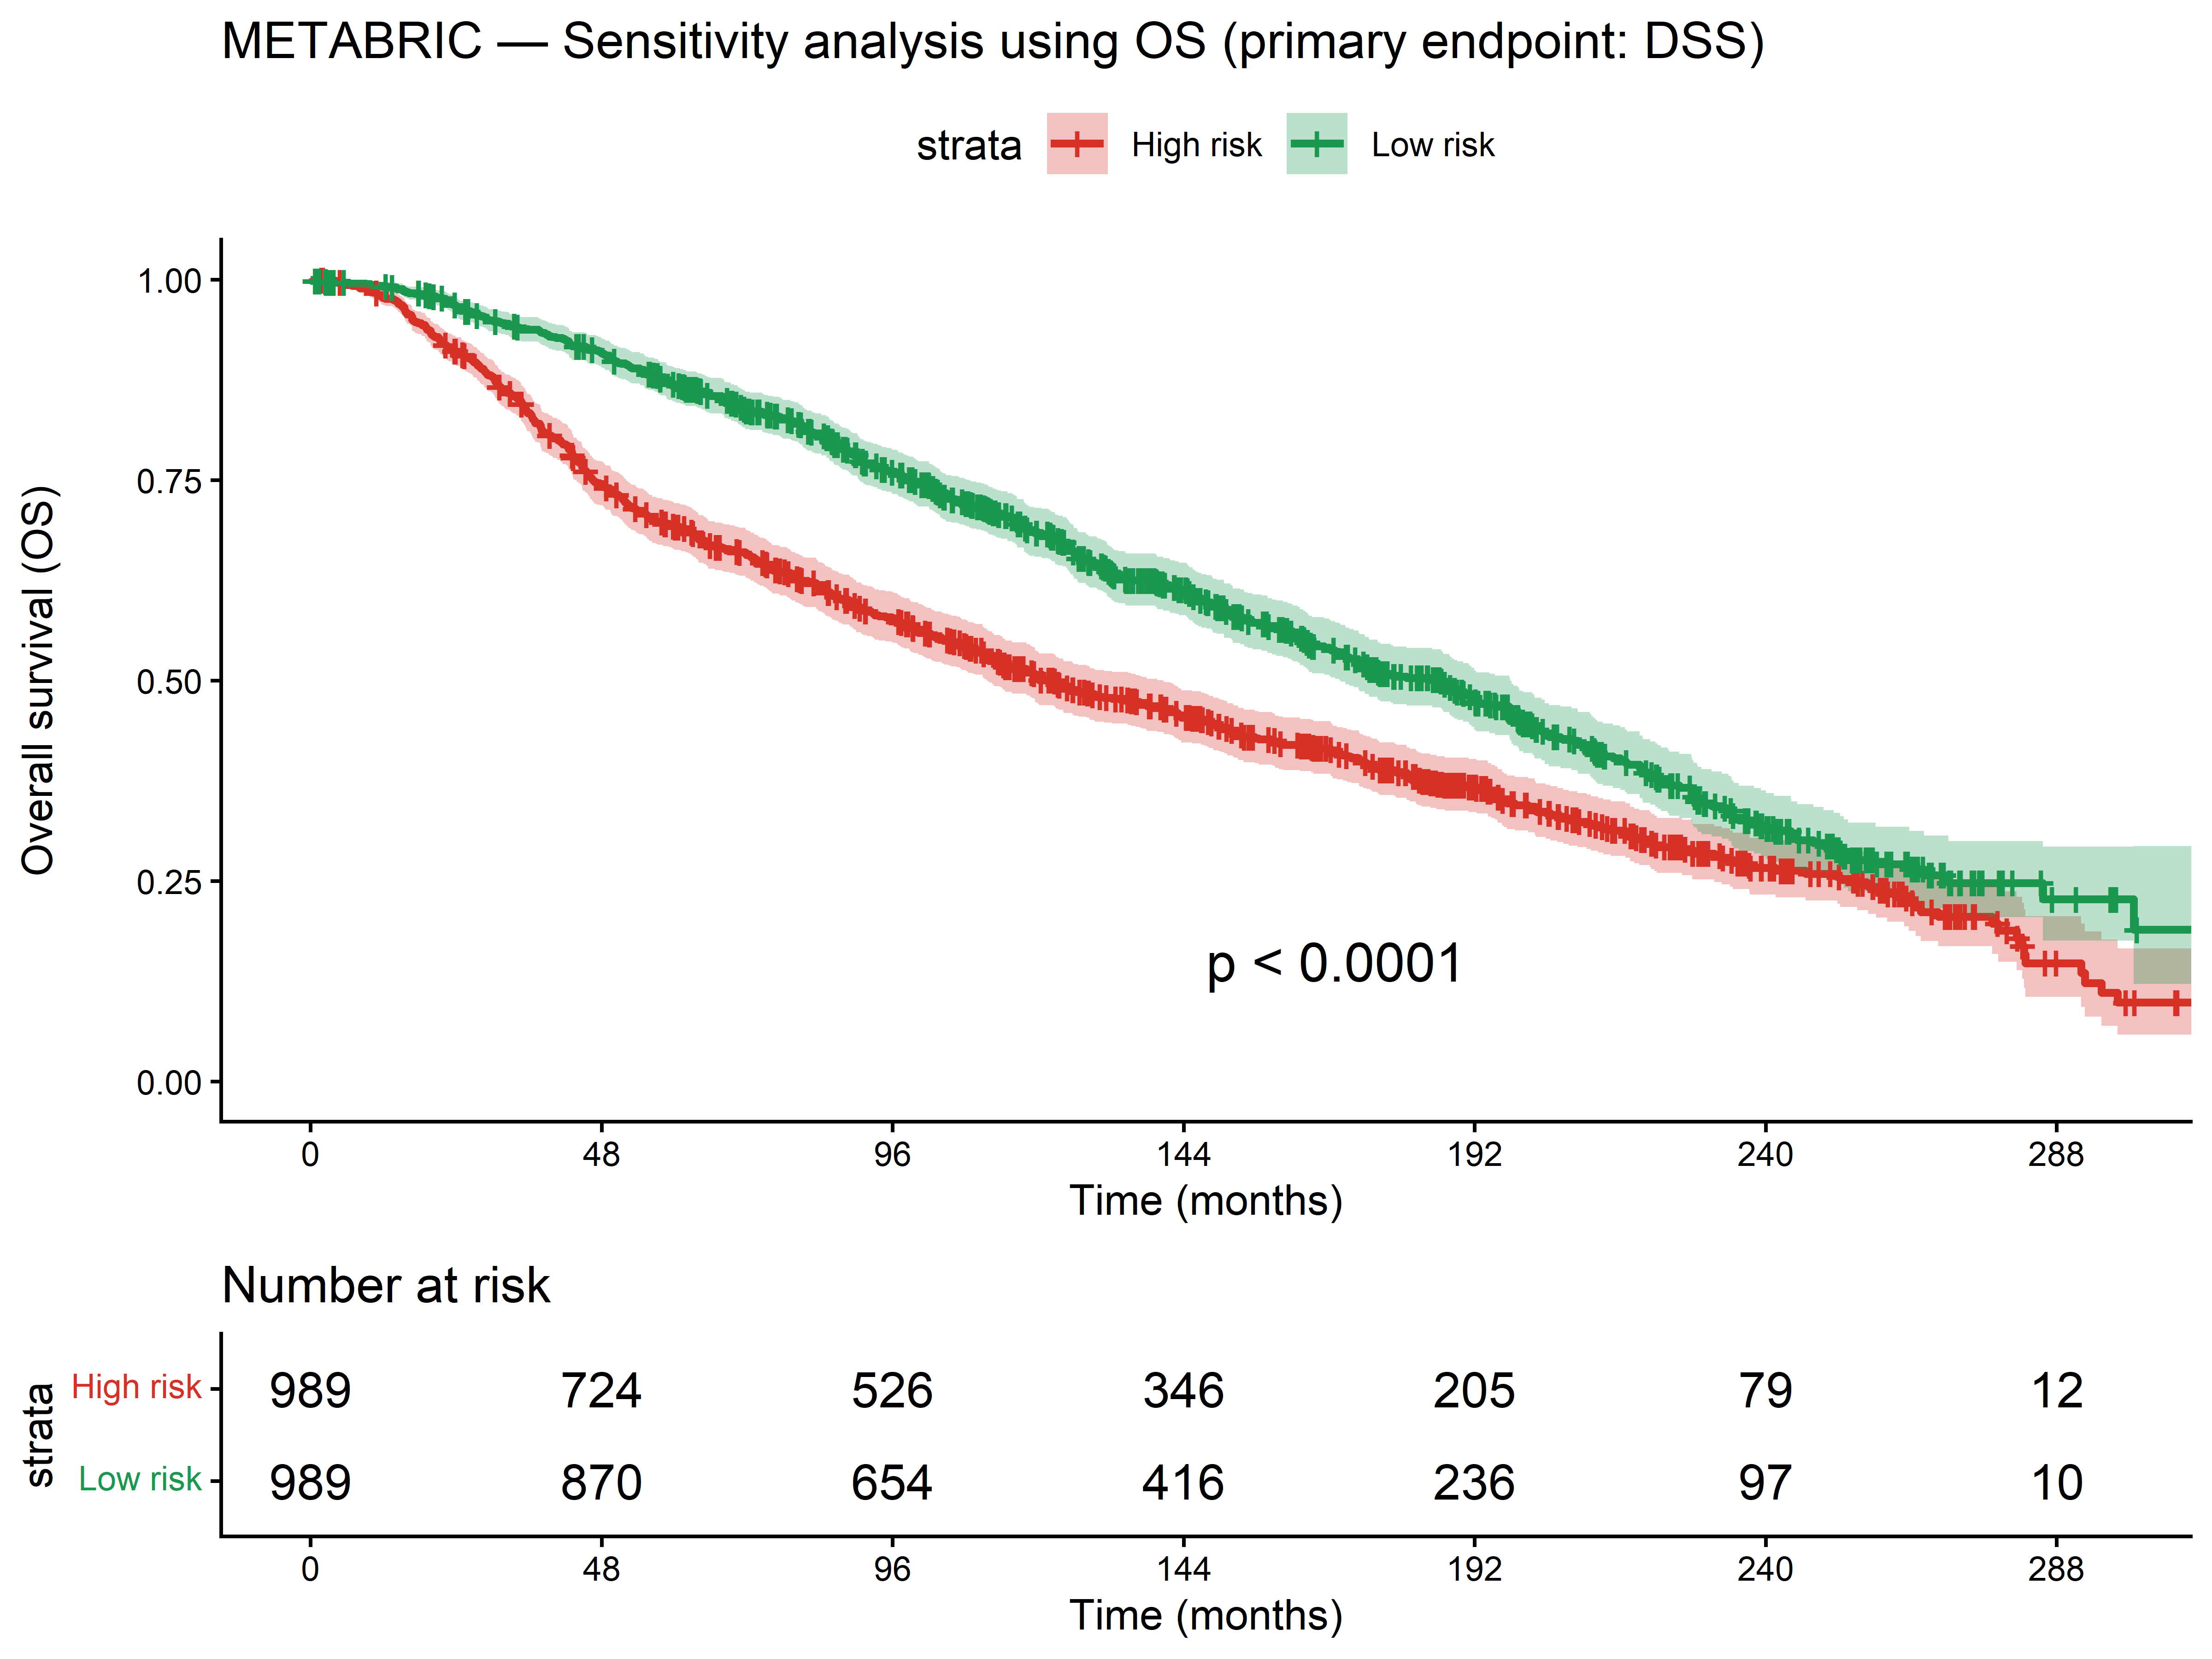
\includegraphics[width=\textwidth,height=0.85\textheight,keepaspectratio]{additional_files/Additional_file_05_FigS5_METABRIC_Sensitivity.png}
\caption{\textbf{Additional file~5: Figure~S5.} METABRIC sensitivity analyses. A: OS endpoint. B: Fine--Gray competing risks model. C: Quartile Kaplan--Meier (DSS).}\label{fig:s5-metabric-sens}
\end{figure}

%% --- Figure S6 ---
\begin{figure}[p]
\centering
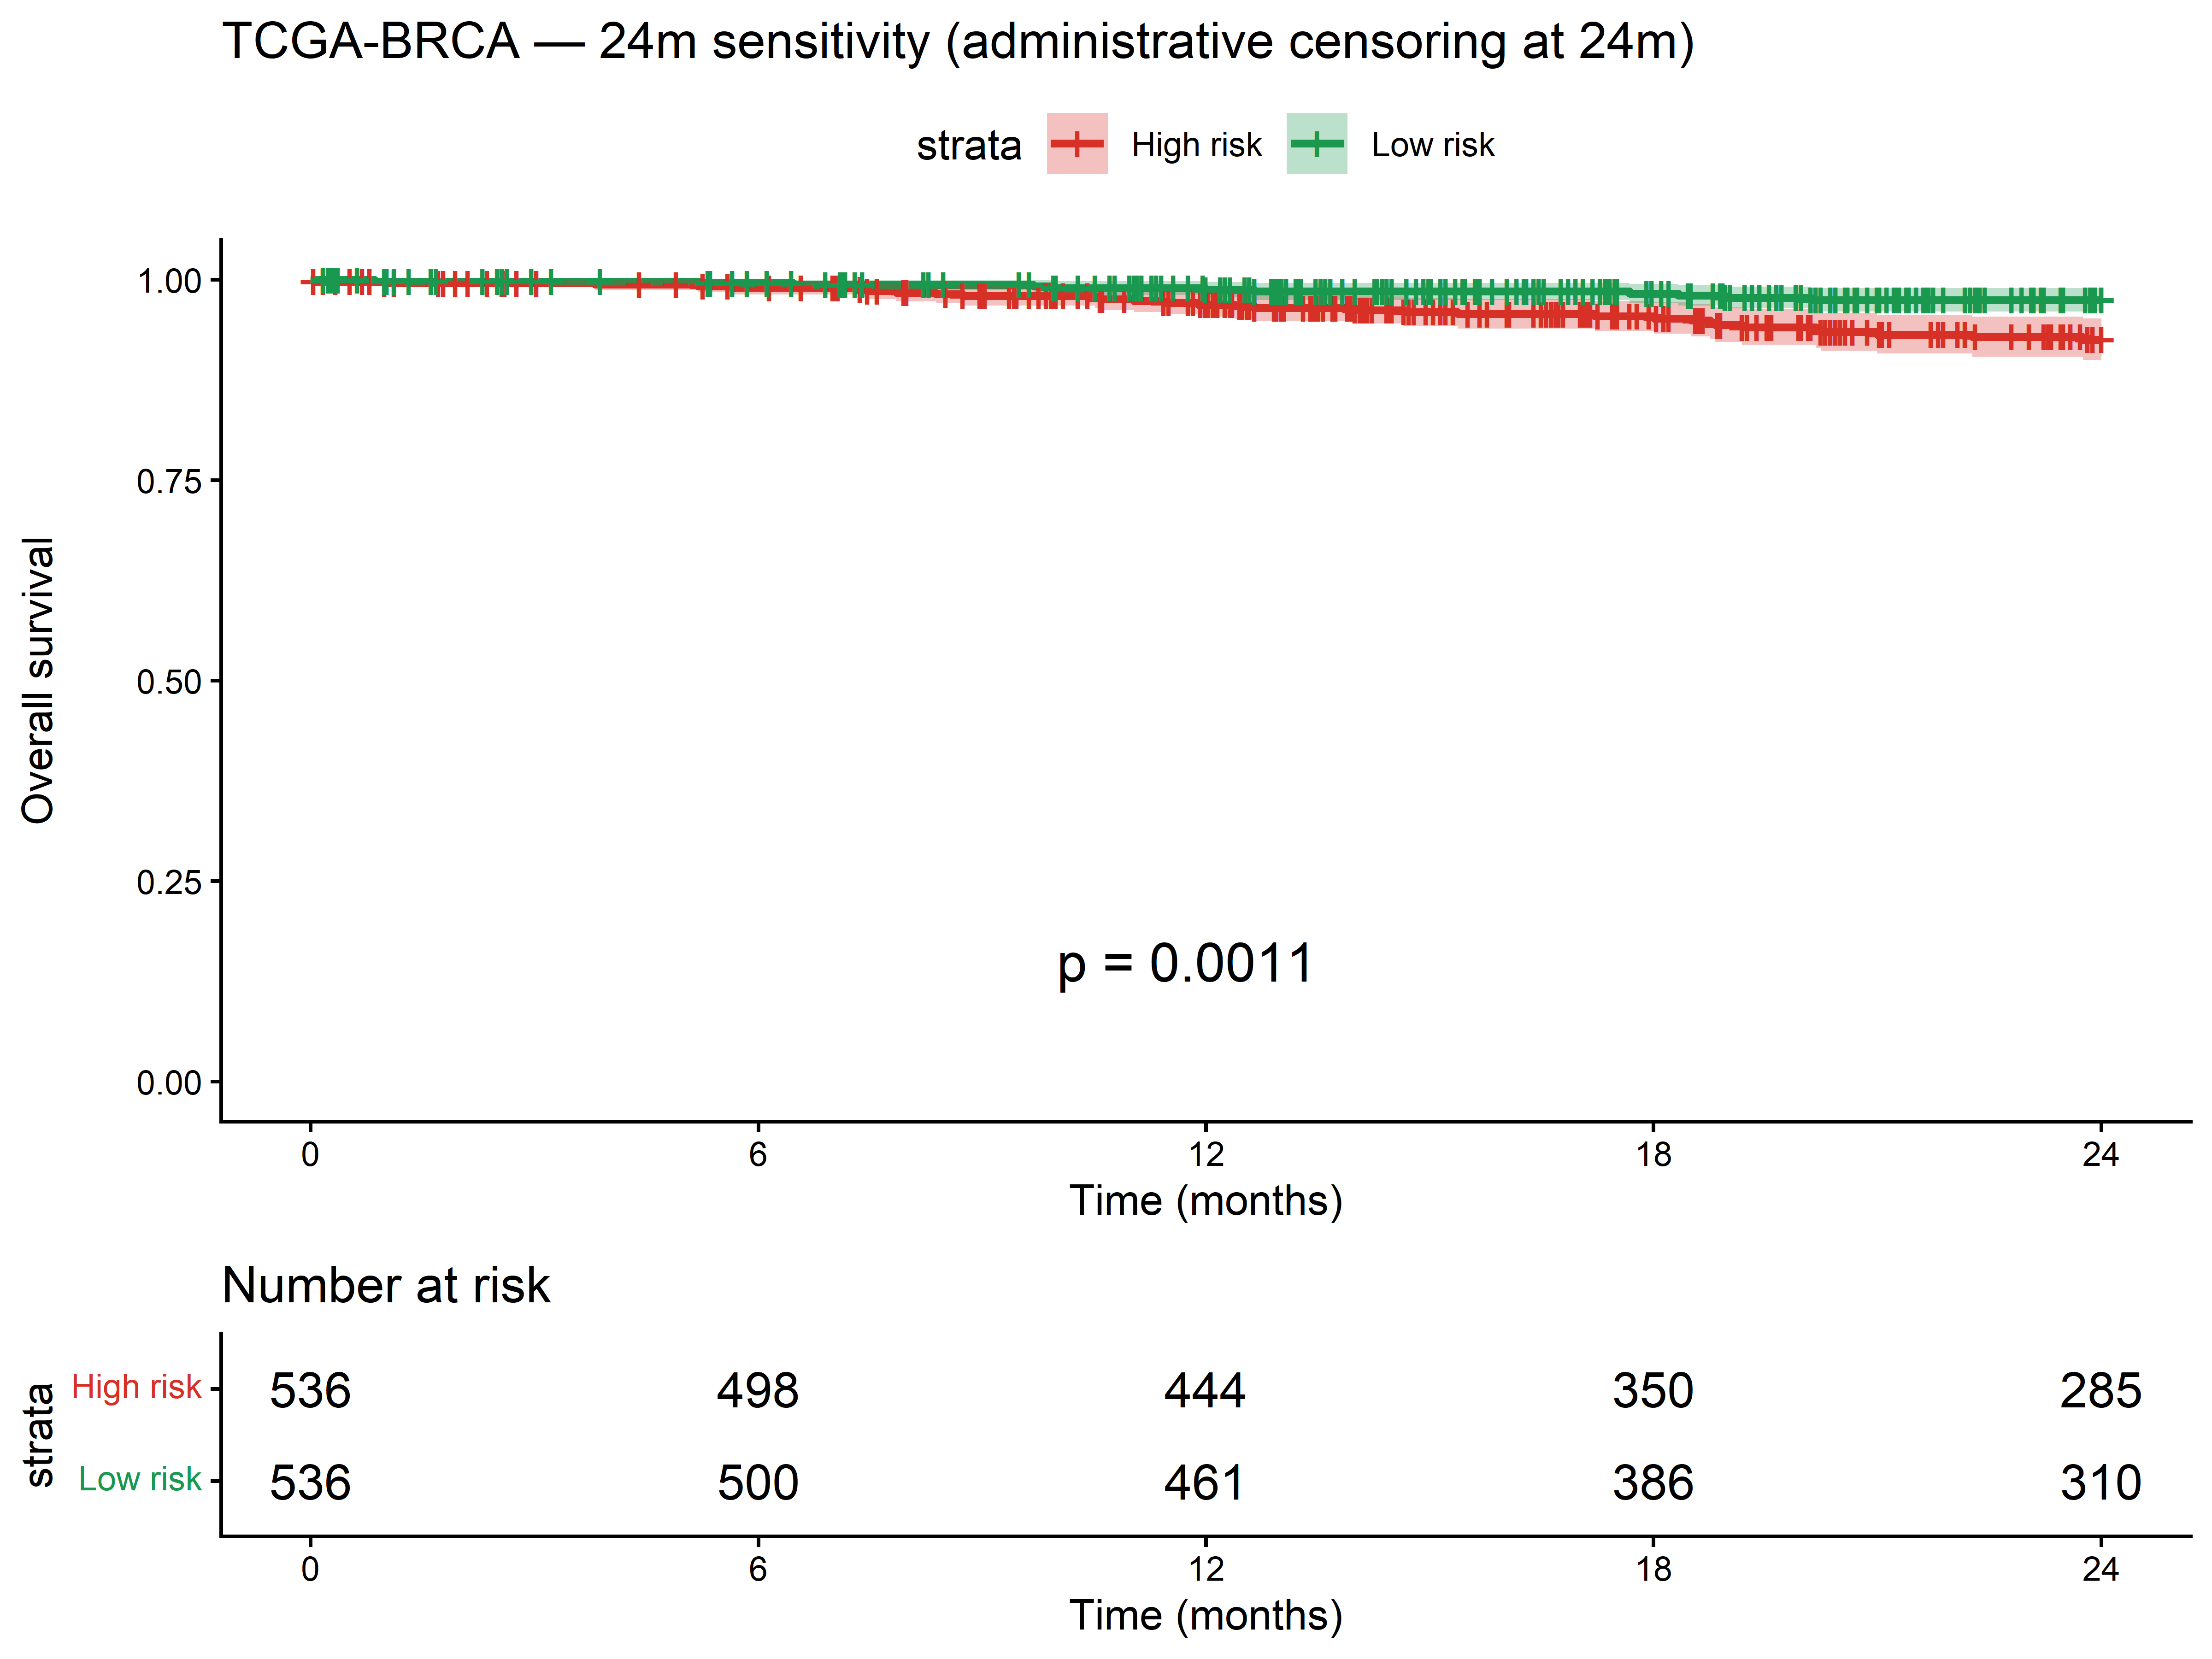
\includegraphics[width=\textwidth,height=0.85\textheight,keepaspectratio]{additional_files/Additional_file_06_FigS6_TCGA_24m.png}
\caption{\textbf{Additional file~6: Figure~S6.} TCGA-BRCA 24-month sensitivity analysis.}\label{fig:s6-tcga-24m}
\end{figure}

%% --- Figure S7 ---
\begin{figure}[p]
\centering
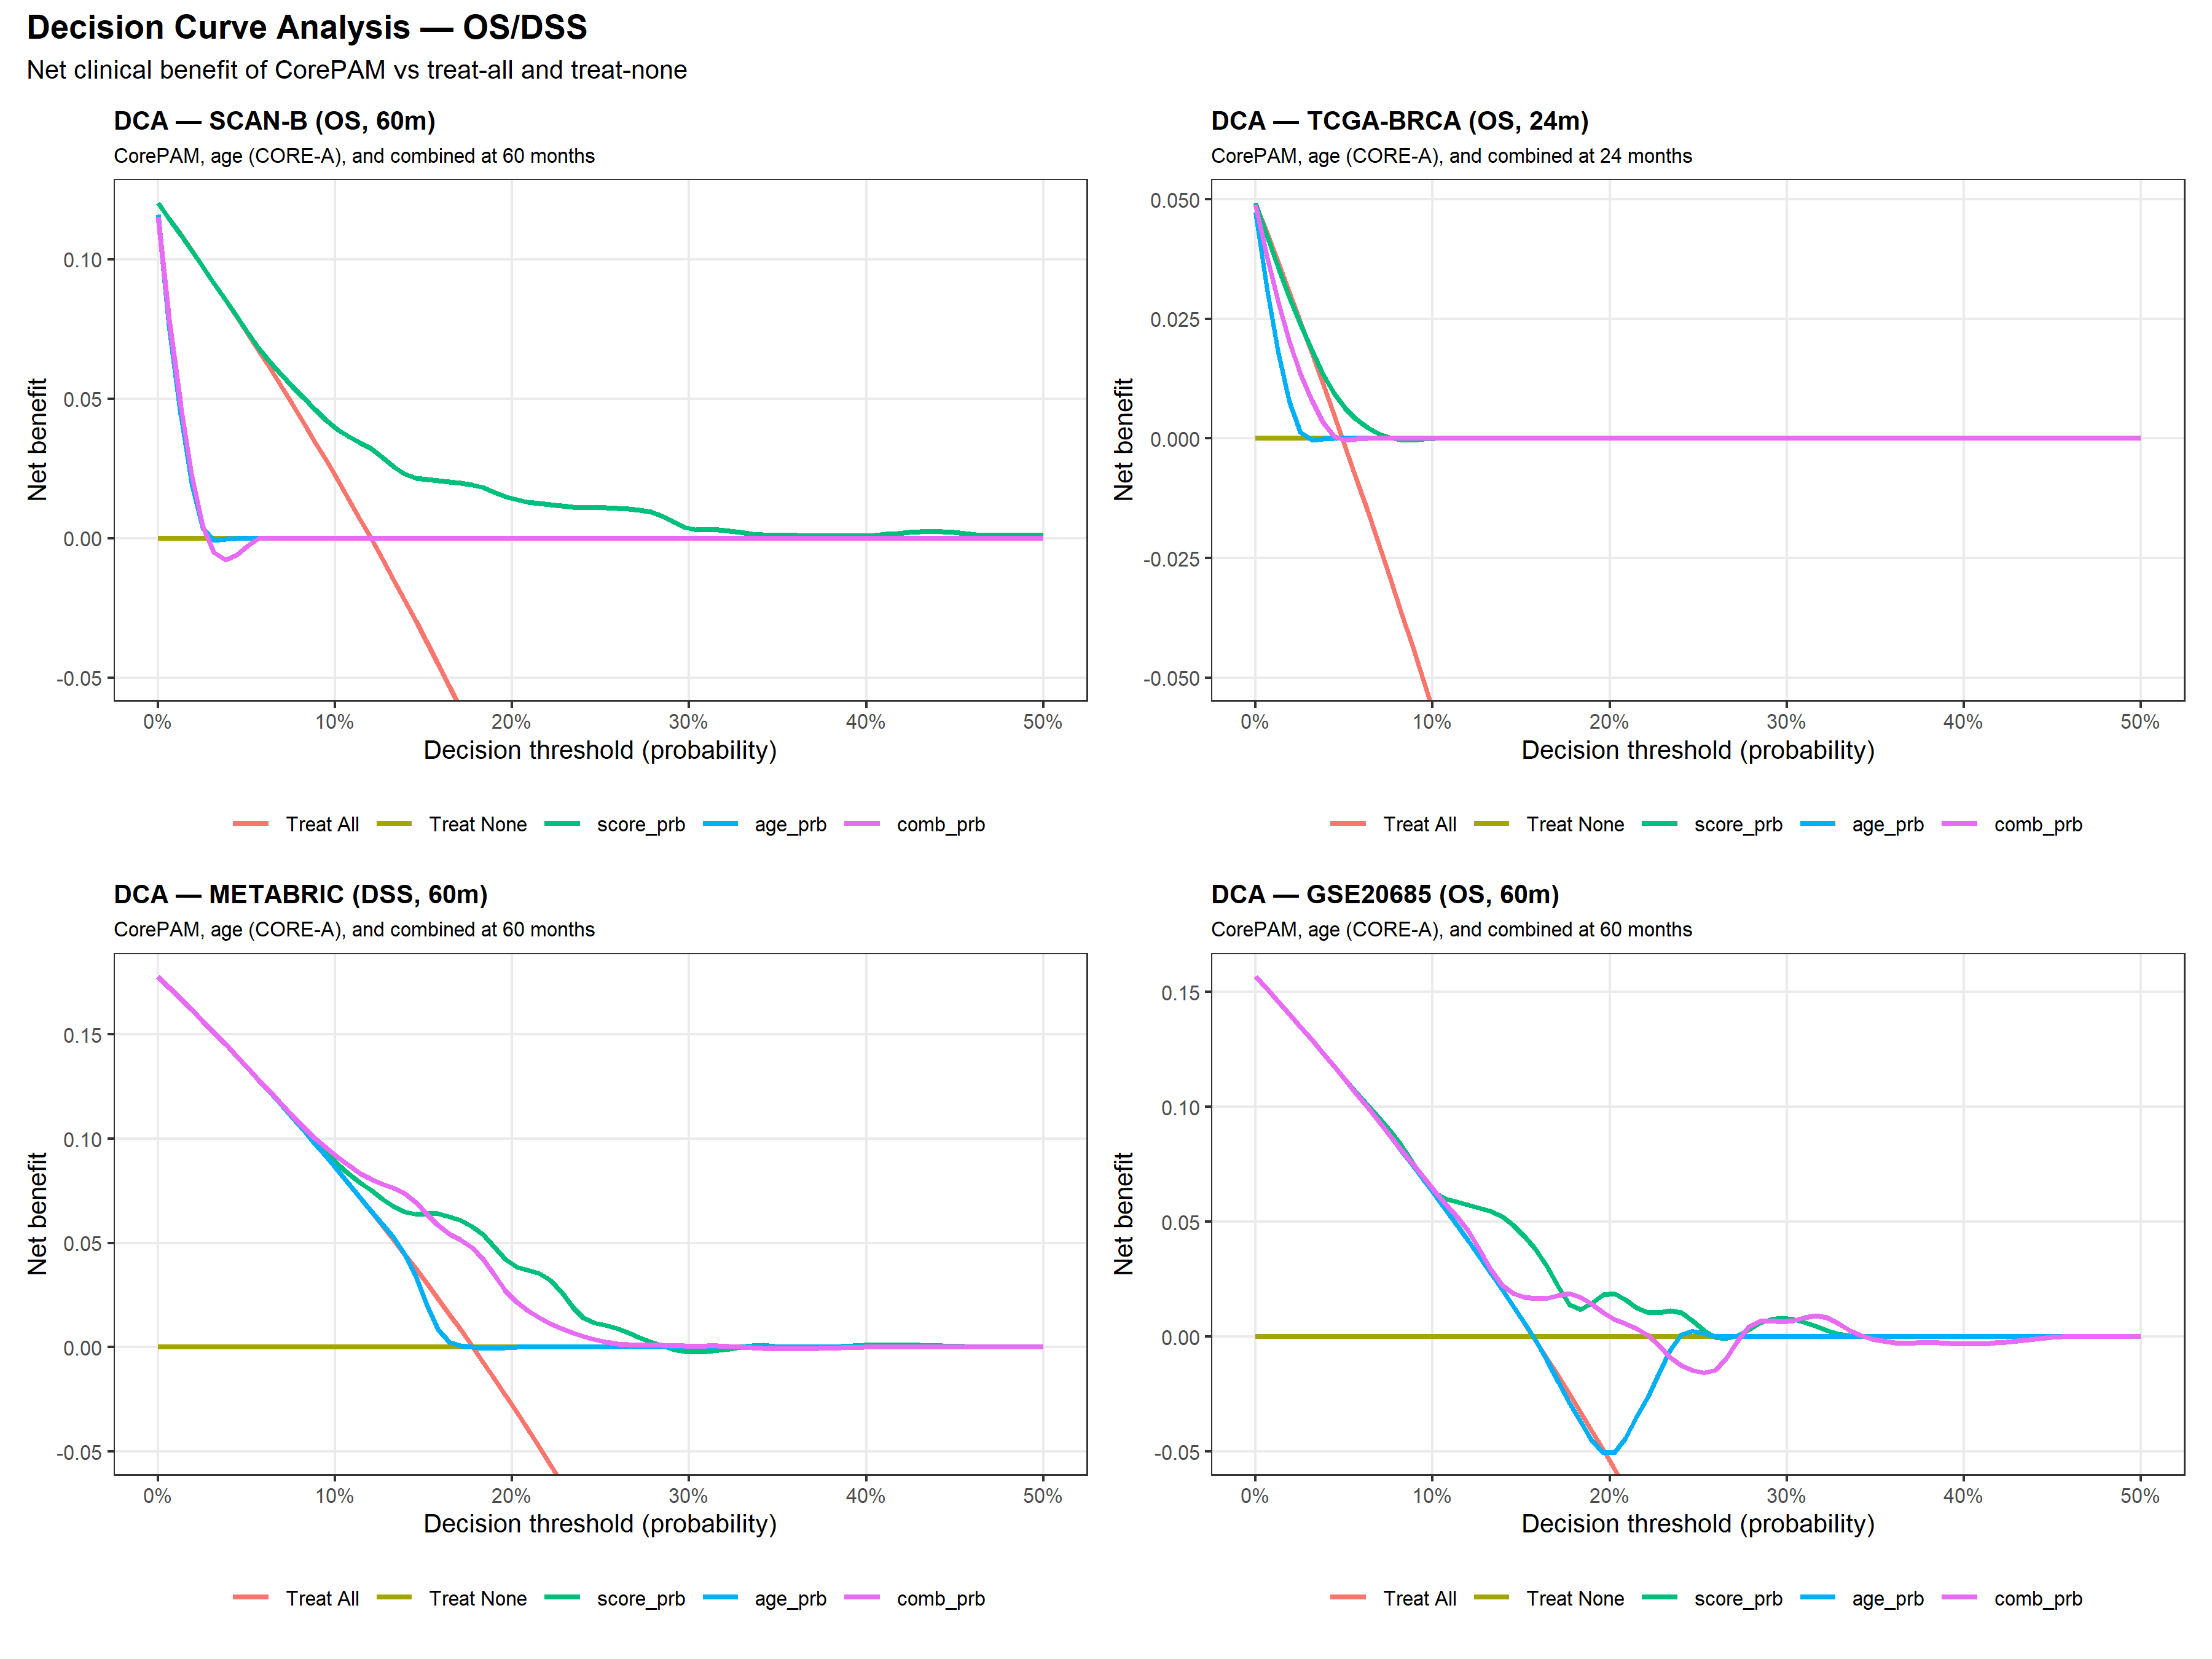
\includegraphics[width=\textwidth,height=0.85\textheight,keepaspectratio]{additional_files/Additional_file_07_FigS7_DCA_OS.png}
\caption{\textbf{Additional file~7: Figure~S7.} Decision curve analysis (OS). Net benefit versus treat-all and treat-none strategies. Horizons: 60 months (SCAN-B, METABRIC, GSE20685) and 24 months (TCGA-BRCA).}\label{fig:s7-dca}
\end{figure}

%% --- Figure S8 ---
\begin{figure}[p]
\centering
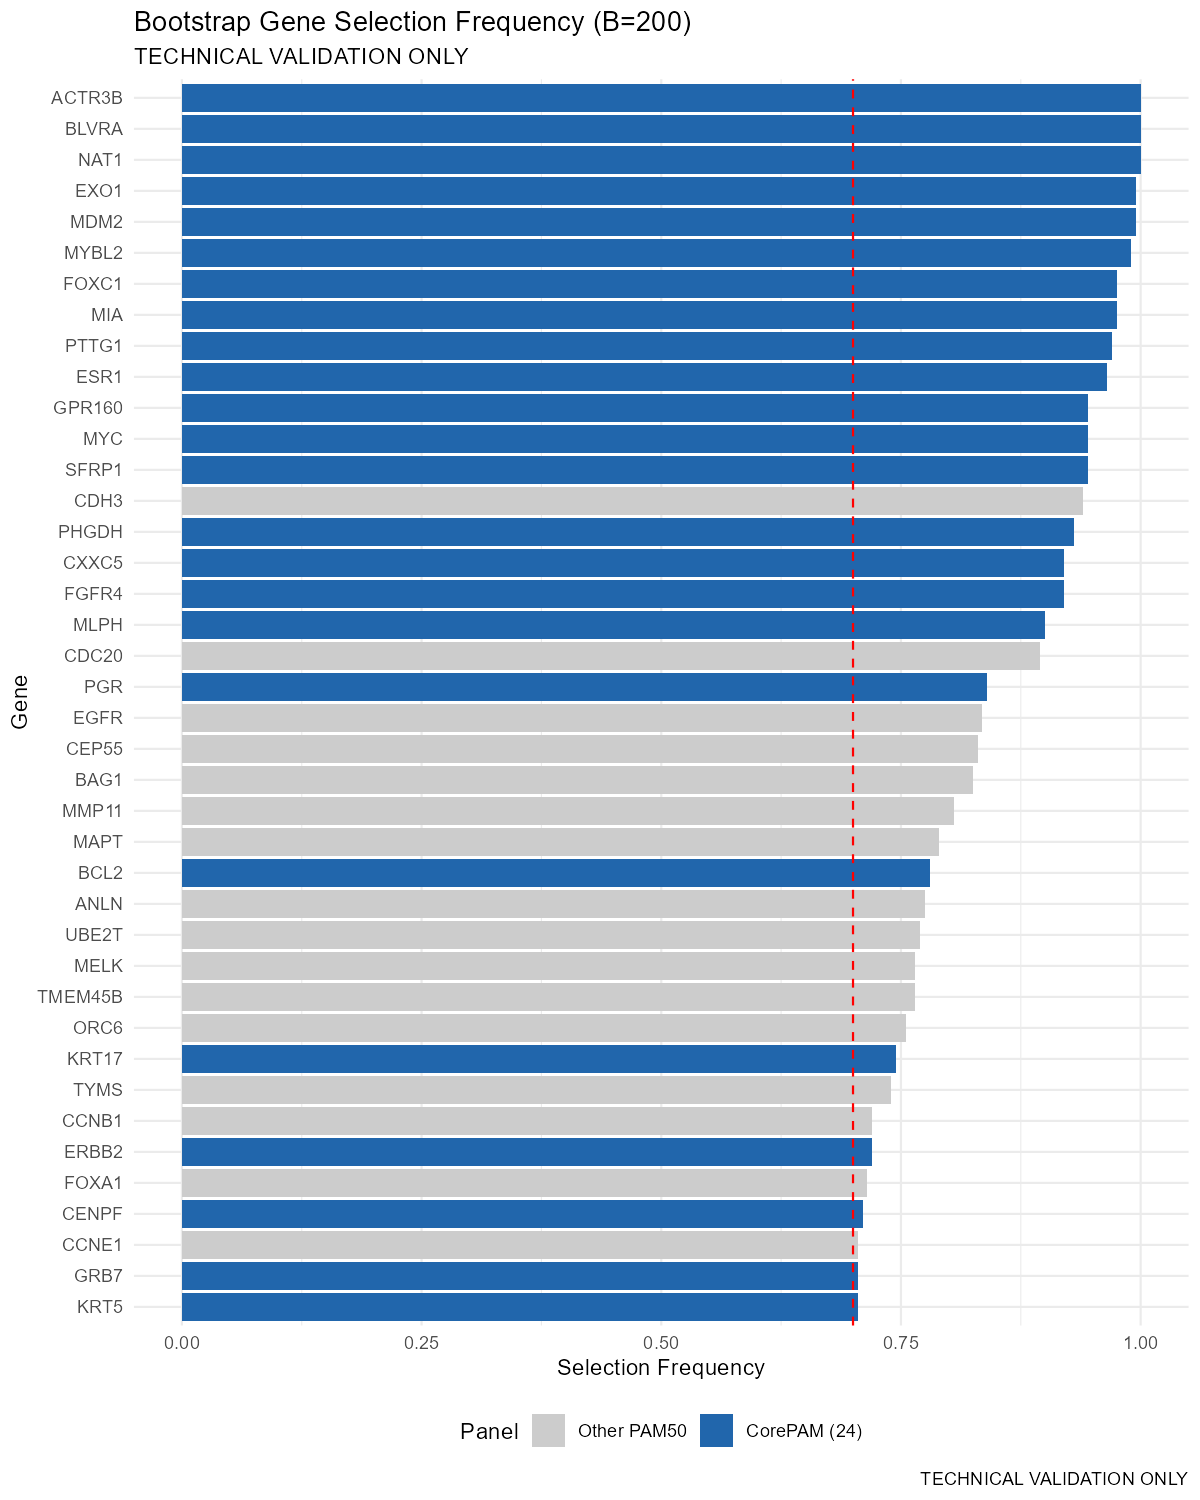
\includegraphics[width=\textwidth,height=0.85\textheight,keepaspectratio]{additional_files/Additional_file_08_FigS8_Bootstrap.png}
\caption{\textbf{Additional file~8: Figure~S8.} Bootstrap stability of CorePAM gene selection ($B = 200$). Frequency of each PAM50 gene across 200 bootstrap refits.}\label{fig:s8-bootstrap}
\end{figure}

%% --- Figure S9 ---
\begin{figure}[p]
\centering
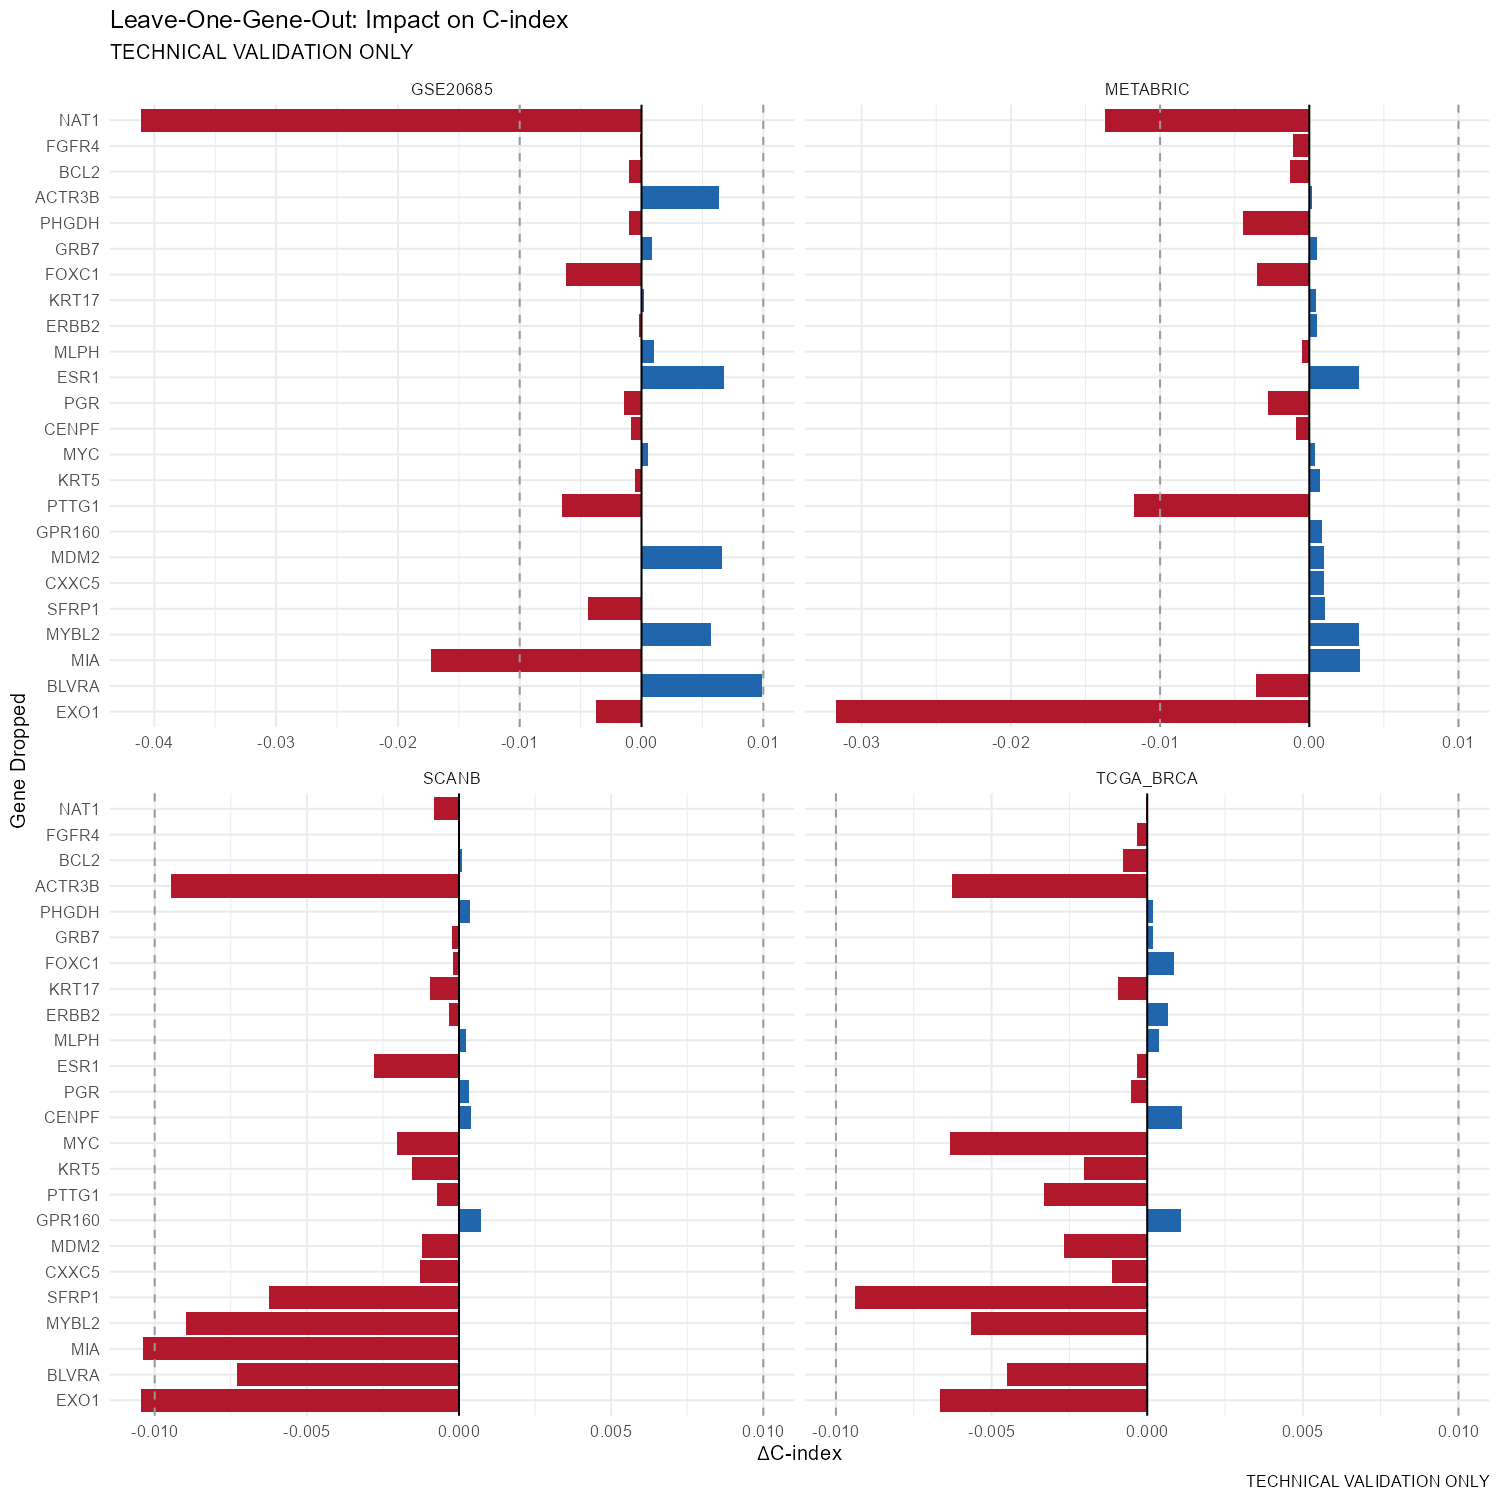
\includegraphics[width=\textwidth,height=0.85\textheight,keepaspectratio]{additional_files/Additional_file_09_FigS9_GeneDropout.png}
\caption{\textbf{Additional file~9: Figure~S9.} Leave-one-gene-out sensitivity analysis. Change in C-index when each CorePAM gene is individually removed.}\label{fig:s9-dropout}
\end{figure}

%% --- Figure S10 ---
\begin{figure}[p]
\centering
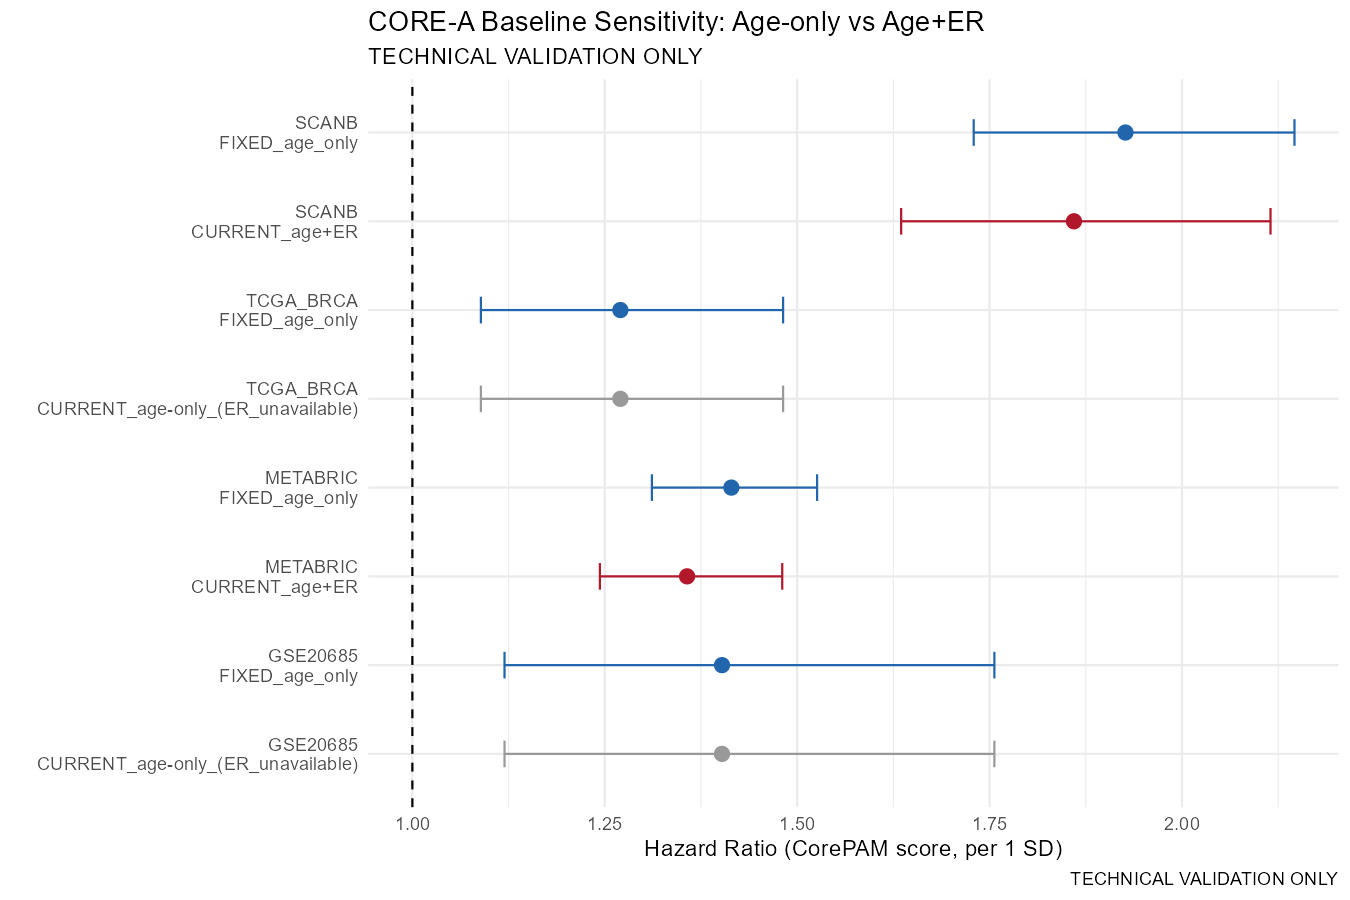
\includegraphics[width=\textwidth,height=0.85\textheight,keepaspectratio]{additional_files/Additional_file_10_FigS10_COREA_Sensitivity.png}
\caption{\textbf{Additional file~10: Figure~S10.} CORE-A baseline sensitivity analysis. Forest plot comparing CorePAM adjusted HR under different clinical baselines.}\label{fig:s10-corea-sens}
\end{figure}

%% --- Table S1: Gene weights ---
\begin{table}[h]
\caption{\textbf{Additional file~11: Table~S1.} CorePAM gene list with elastic-net Cox regression weights (24 genes). Positive weights: higher expression associated with worse survival; negative weights: protective association.}\label{tab:s1-weights}
\begin{tabular}{@{}lrl@{}}
\toprule
Gene & Weight & Direction \\
\midrule
EXO1 & 0.2174 & Risk (+) \\
NAT1 & $-$0.2052 & Protective ($-$) \\
BLVRA & $-$0.1848 & Protective ($-$) \\
ACTR3B & $-$0.1405 & Protective ($-$) \\
MIA & $-$0.1193 & Protective ($-$) \\
MYBL2 & $-$0.1183 & Protective ($-$) \\
PTTG1 & 0.1140 & Risk (+) \\
MDM2 & $-$0.1074 & Protective ($-$) \\
SFRP1 & $-$0.0907 & Protective ($-$) \\
GPR160 & $-$0.0841 & Protective ($-$) \\
FOXC1 & 0.0717 & Risk (+) \\
PHGDH & 0.0620 & Risk (+) \\
MYC & $-$0.0424 & Protective ($-$) \\
ESR1 & 0.0396 & Risk (+) \\
KRT5 & $-$0.0277 & Protective ($-$) \\
CXXC5 & 0.0266 & Risk (+) \\
PGR & $-$0.0262 & Protective ($-$) \\
KRT17 & $-$0.0163 & Protective ($-$) \\
CENPF & 0.0150 & Risk (+) \\
FGFR4 & 0.0110 & Risk (+) \\
BCL2 & $-$0.0105 & Protective ($-$) \\
MLPH & $-$0.0099 & Protective ($-$) \\
ERBB2 & $-$0.0082 & Protective ($-$) \\
GRB7 & $-$0.0053 & Protective ($-$) \\
\botrule
\end{tabular}
\end{table}

%% --- Table S2: Expanded CORE-A ---
\begin{table}[h]
\caption{\textbf{Additional file~12: Table~S2.} Expanded CORE-A analysis: CorePAM independence from anatomical staging (T-stage, nodal status). HR per 1~SD CorePAM score from multivariable Cox regression.}\label{tab:s2-expanded}
\begin{tabular}{@{}lrlllrrr@{}}
\toprule
Cohort & N & Covariates & HR (95\% CI) & $p$ & C clin & C clin+score & $\Delta$C \\
\midrule
SCAN-B & 2,948 & age+ER+T+N & 1.79 (1.57--2.05) & $<$0.001 & 0.766 & 0.788 & +0.022 \\
TCGA-BRCA & 1,054 & age+T+N & 1.35 (1.15--1.58) & $<$0.001 & 0.719 & 0.746 & +0.027 \\
METABRIC & 1,883 & age+ER+T+N & 1.34 (1.23--1.46) & $<$0.001 & 0.663 & 0.688 & +0.026 \\
GSE20685 & 327 & age+T+N & 1.47 (1.15--1.86) & 0.002 & 0.697 & 0.722 & +0.025 \\
\botrule
\end{tabular}
\end{table}

%% --- Table S3: Genefu comparison ---
\begin{table}[h]
\caption{\textbf{Additional file~13: Table~S3.} Head-to-head C-index comparison: CorePAM (24 genes) vs research-based ROR-S (50 genes) and OncotypeDX-RS (21 genes). All scores per 1~SD.}\label{tab:s3-genefu}
\begin{tabular}{@{}lrcccccc@{}}
\toprule
Cohort & N & CorePAM C & ROR-S C & ODX-RS C & CorePAM HR & ROR-S HR & ODX-RS HR \\
\midrule
SCAN-B & 3,069 & 0.698 & 0.641 & 0.607 & 1.92 & 1.56 & 1.40 \\
TCGA-BRCA & 1,072 & 0.624 & 0.602 & 0.586 & 1.20 & 1.25 & 1.13 \\
METABRIC & 1,978 & 0.638 & 0.643 & 0.665 & 1.41 & 1.53 & 1.51 \\
GSE20685 & 327 & 0.623 & 0.647 & 0.648 & 1.40 & 1.57 & 1.59 \\
\botrule
\end{tabular}
\end{table}

%% --- Table S4: Frozen z-score sensitivity ---
\begin{table}[h]
\caption{\textbf{Additional file~14: Table~S4.} Frozen z-score sensitivity analysis. C-index and Pearson correlation ($r$) between frozen and intra-cohort scoring approaches. \textbf{Note:} HRs in this table are per unit of raw weighted score (no cohort-level re-standardisation) and are therefore \textbf{not directly comparable} to the per-1-SD HRs in Table~\ref{tab:survival}. The relevant comparison metric is the C-index, which is rank-invariant across scoring scales.}\label{tab:s4-frozen}
\small
\begin{tabular}{@{}lrccccc@{}}
\toprule
Cohort & N & Platform & C frozen & C intra & $\Delta$C & $r$ \\
\midrule
SCAN-B & 3,069 & RNA-seq & 0.698 & 0.698 & 0.0000 & 1.000 \\
TCGA-BRCA & 1,072 & RNA-seq & 0.624 & 0.624 & +0.0002 & 0.999 \\
METABRIC & 1,978 & Microarray & 0.638 & 0.638 & +0.0007 & 0.958 \\
GSE20685 & 327 & Microarray & 0.581 & 0.623 & $-$0.042 & 0.921 \\
\botrule
\end{tabular}
\footnotetext{C frozen/intra: Harrell's C-index under frozen (SCAN-B reference) vs intra-cohort z-score normalisation. $\Delta$C = C(frozen) $-$ C(intra). $r$: Pearson correlation between frozen and intra-cohort scores. C-index is rank-invariant and directly comparable across scoring scales.}
\end{table}

%% --- Table S5: Uno's C + tdAUC ---
\begin{table}[h]
\caption{\textbf{Additional file~15: Table~S5.} Uno's C-statistic (IPCW) and time-dependent AUC at cohort-specific horizons.}\label{tab:s5-unoc}
\begin{tabular}{@{}lrrccc@{}}
\toprule
Cohort & N & Horizon & Uno's C & tdAUC (95\% CI) & Harrell's C \\
\midrule
SCAN-B & 3,069 & 60m & 0.674 & 0.679 (0.643--0.715) & 0.698 \\
TCGA-BRCA & 1,072 & 24m & 0.669 & 0.673 (0.598--0.748) & 0.624 \\
METABRIC & 1,978 & 60m & 0.681 & 0.695 (0.665--0.725) & 0.638 \\
GSE20685 & 327 & 60m & 0.663 & 0.671 (0.592--0.750) & 0.623 \\
\botrule
\end{tabular}
\end{table}

%% --- Table S6: Formal calibration ---
\begin{table}[h]
\caption{\textbf{Additional file~16: Table~S6.} Formal calibration: logistic recalibration intercept ($\alpha$) and slope ($\beta$) at cohort-specific horizons. Ideal: $\alpha = 0$, $\beta = 1$.}\label{tab:s6-calibration}
\begin{tabular}{@{}lrrcccc@{}}
\toprule
Cohort & N & Horizon & $\alpha$ (SE) & $\beta$ (SE) & E/O & Brier \\
\midrule
SCAN-B & 3,069 & 60m & 0.56 (0.18) & 0.96 (0.09) & 0.61 & 0.158 \\
TCGA-BRCA & 1,072 & 24m & 5.40 (2.29) & 2.74 (0.79) & 0.74 & 0.061 \\
METABRIC & 1,978 & 60m & 1.15 (0.25) & 1.77 (0.17) & 0.97 & 0.143 \\
GSE20685 & 327 & 60m & 0.96 (0.75) & 1.58 (0.46) & 0.98 & 0.130 \\
\botrule
\end{tabular}
\end{table}

%% --- Table S7: Full clinical baseline incremental value ---
\begin{table}[h]
\caption{\textbf{Additional file~17: Table~S7.} Full clinical baseline incremental value analysis. Cox regression with six clinical-pathological covariates (age, ER, T-stage, N-status, grade, HER2) $\pm$ CorePAM.}\label{tab:s7-fullbaseline}
\small
\begin{tabular*}{\textwidth}{@{\extracolsep\fill}llrrcccl}
\toprule
Cohort & Population & N & C clinical & C clin+CorePAM & $\Delta$C & HR$_{\text{adj}}$ & LRT $p$ \\
\midrule
SCAN-B (OS) & All & 2,649 & 0.770 & 0.787 & +0.017 & 1.75 & $4.9 \times 10^{-13}$ \\
SCAN-B (OS) & ER+ & 2,450 & 0.770 & 0.784 & +0.014 & 1.68 & $1.1 \times 10^{-10}$ \\
METABRIC (DSS) & All & 1,792 & 0.678 & 0.693 & +0.015 & 1.25 & $6.1 \times 10^{-6}$ \\
METABRIC (DSS) & ER+ & 1,377 & 0.674 & 0.707 & +0.032 & 1.47 & $1.0 \times 10^{-10}$ \\
\botrule
\end{tabular*}
\footnotetext{HR$_{\text{adj}}$: CorePAM HR per 1~SD adjusted for age, ER, T-stage, N-status, grade, HER2. $\Delta$C: bootstrap (B=1,000). LRT: likelihood ratio test for CorePAM addition.}
\end{table}

%% ============================================================
%%  REFERENCES
%% ============================================================
\bibliography{CorePAM_references}

\end{document}
